\section[Data to Monte Carlo comparisons at $\sqrt{s}=2.36$ TeV in
  Minimum Bias events]{Data to Monte Carlo comparisons at $\boldsymbol{\sqrt{s}=2.36}$ TeV in
  Minimum Bias events}
\label{sc:DataVsMCMB2360}

\subsection[Basic $\etmiss$-related distributions]{Basic $\etmissB$-related distributions}
\begin{figure}[h!]
 \centering
 \begin{tabular}{ll}
  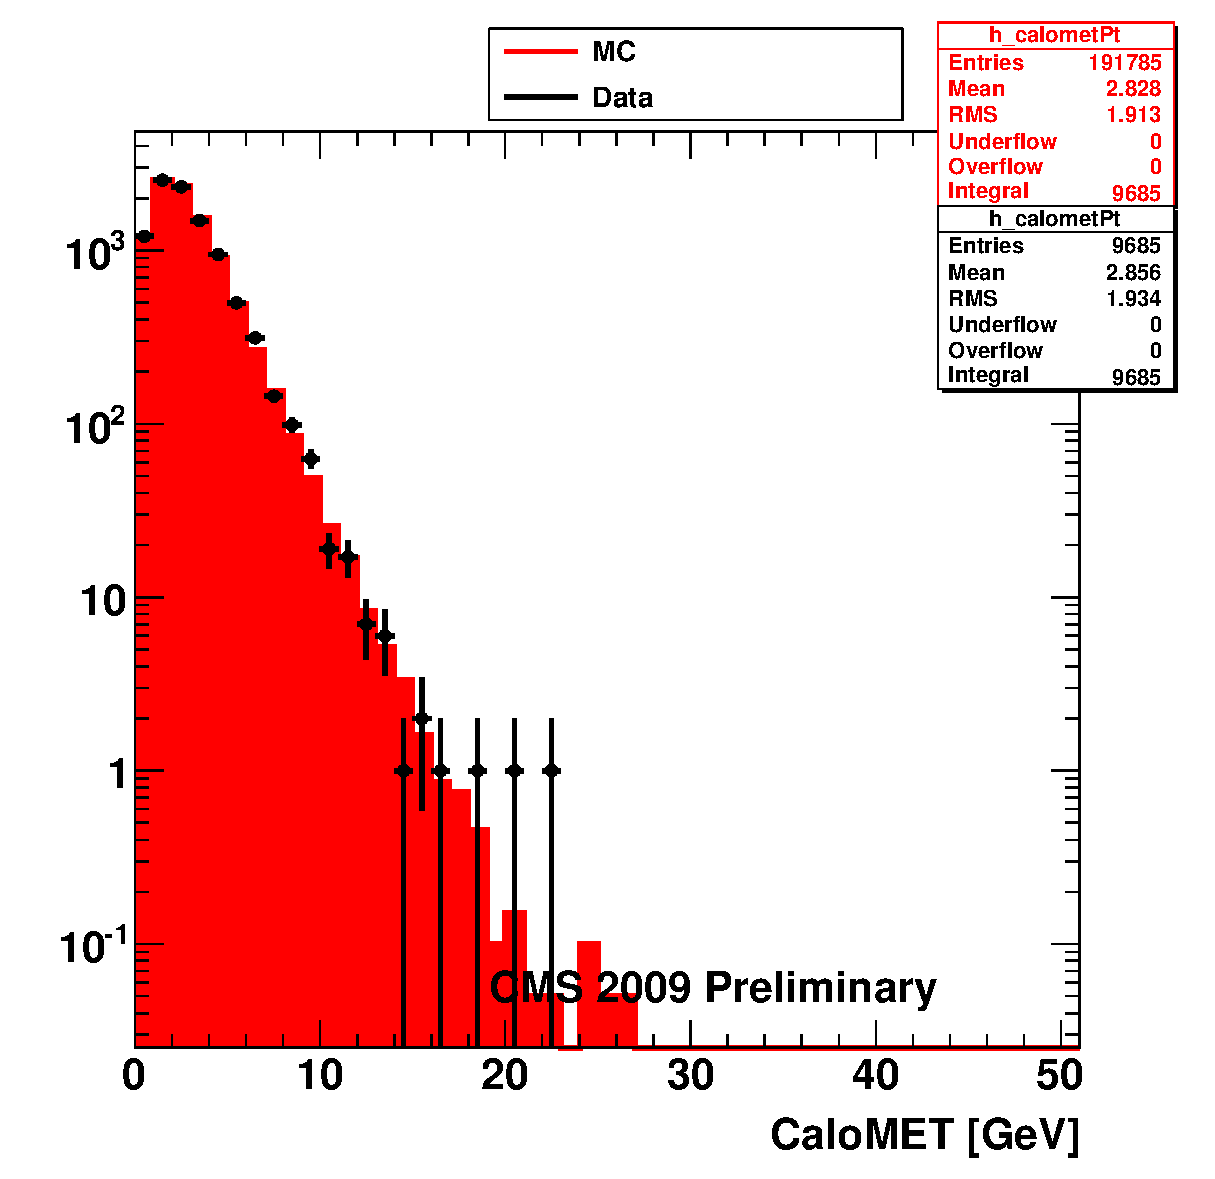
\includegraphics[width=0.40\textwidth]{plots_DataVsMC_MB_2360GeV/h_calometPt.eps} &
  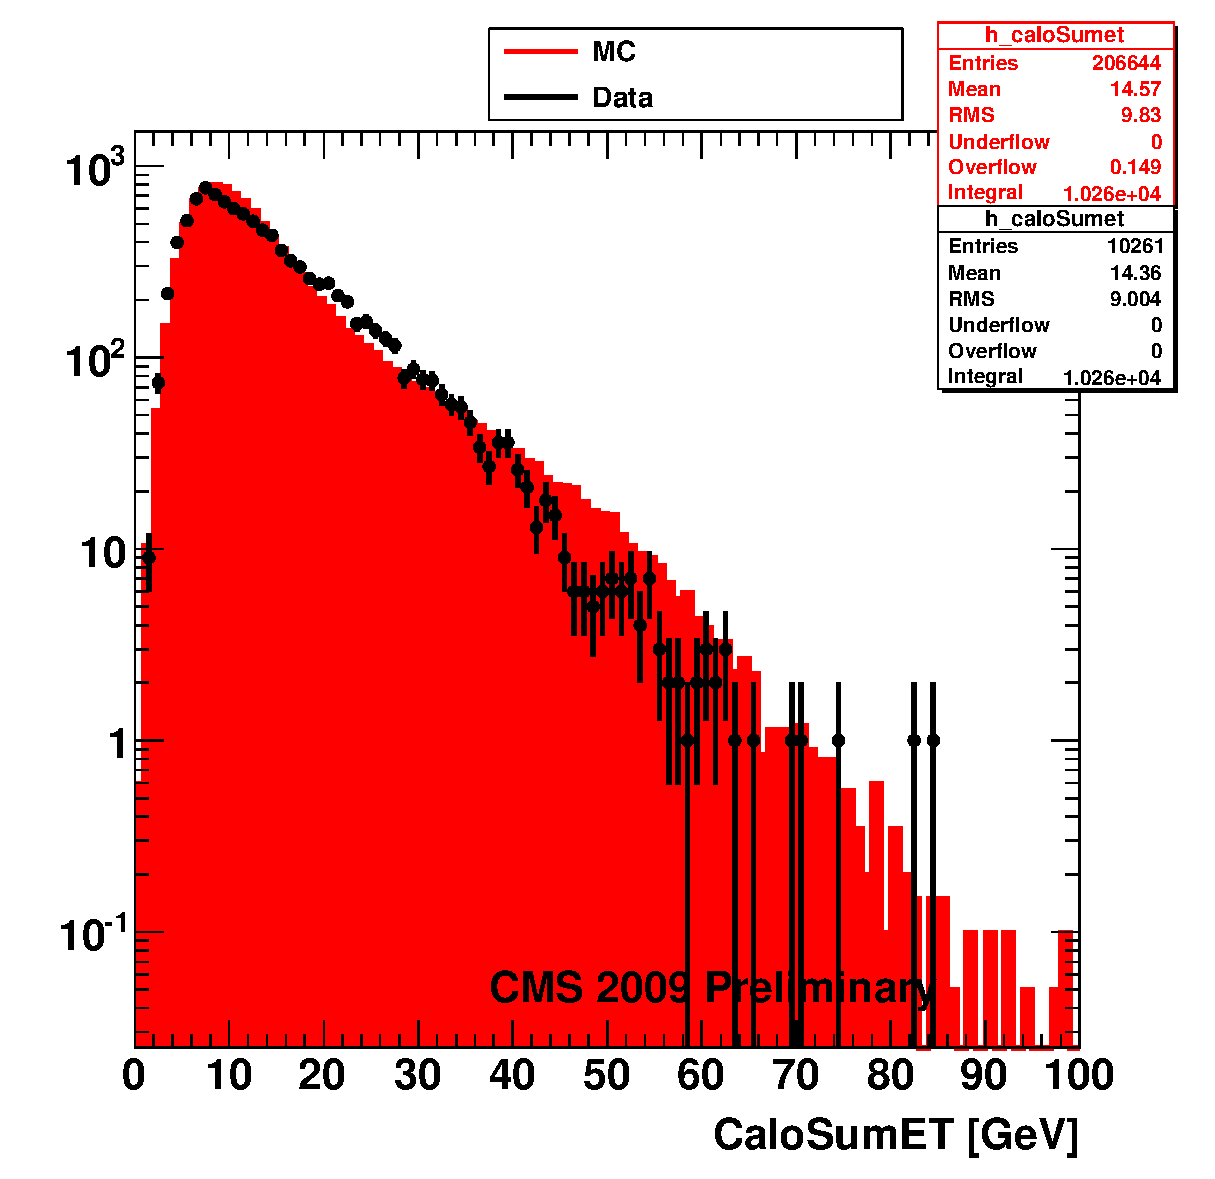
\includegraphics[width=0.40\textwidth]{plots_DataVsMC_MB_2360GeV/h_caloSumet.eps} \\
 \end{tabular}
 \caption{$\etmiss$ and $\sumet$ distributions in 2360 GeV data compared with Monte Carlo simulation.
          \label{fig:DataVsMC_MB_2360_1}}
\end{figure}

\begin{figure}[h!]
 \centering
 \begin{tabular}{ll}
  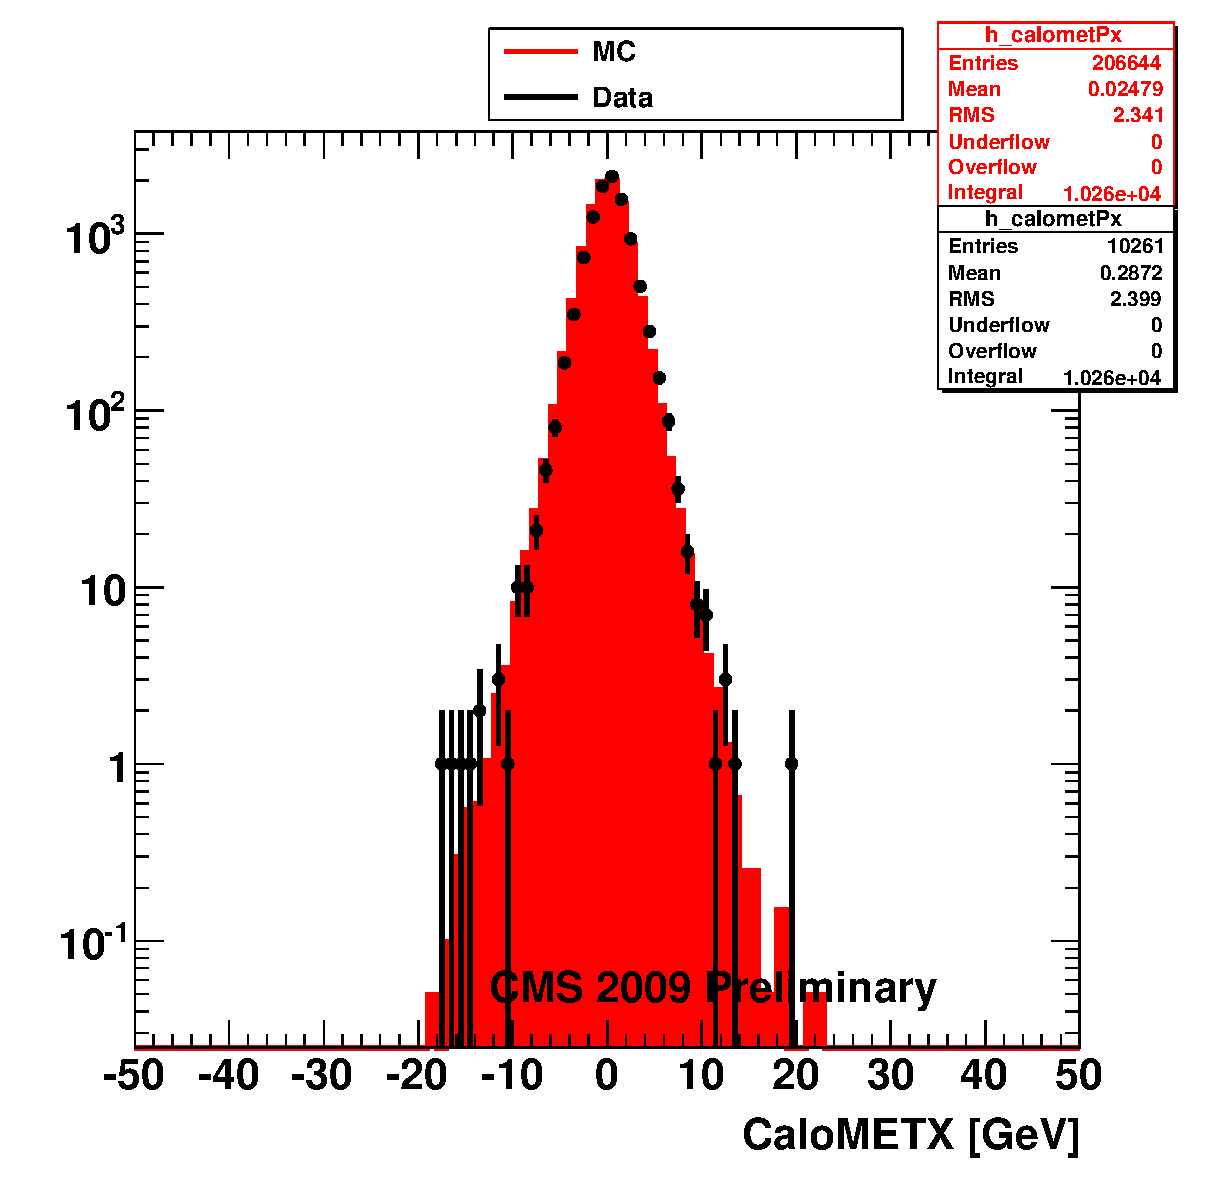
\includegraphics[width=0.40\textwidth]{plots_DataVsMC_MB_2360GeV/h_calometPx.eps} &
  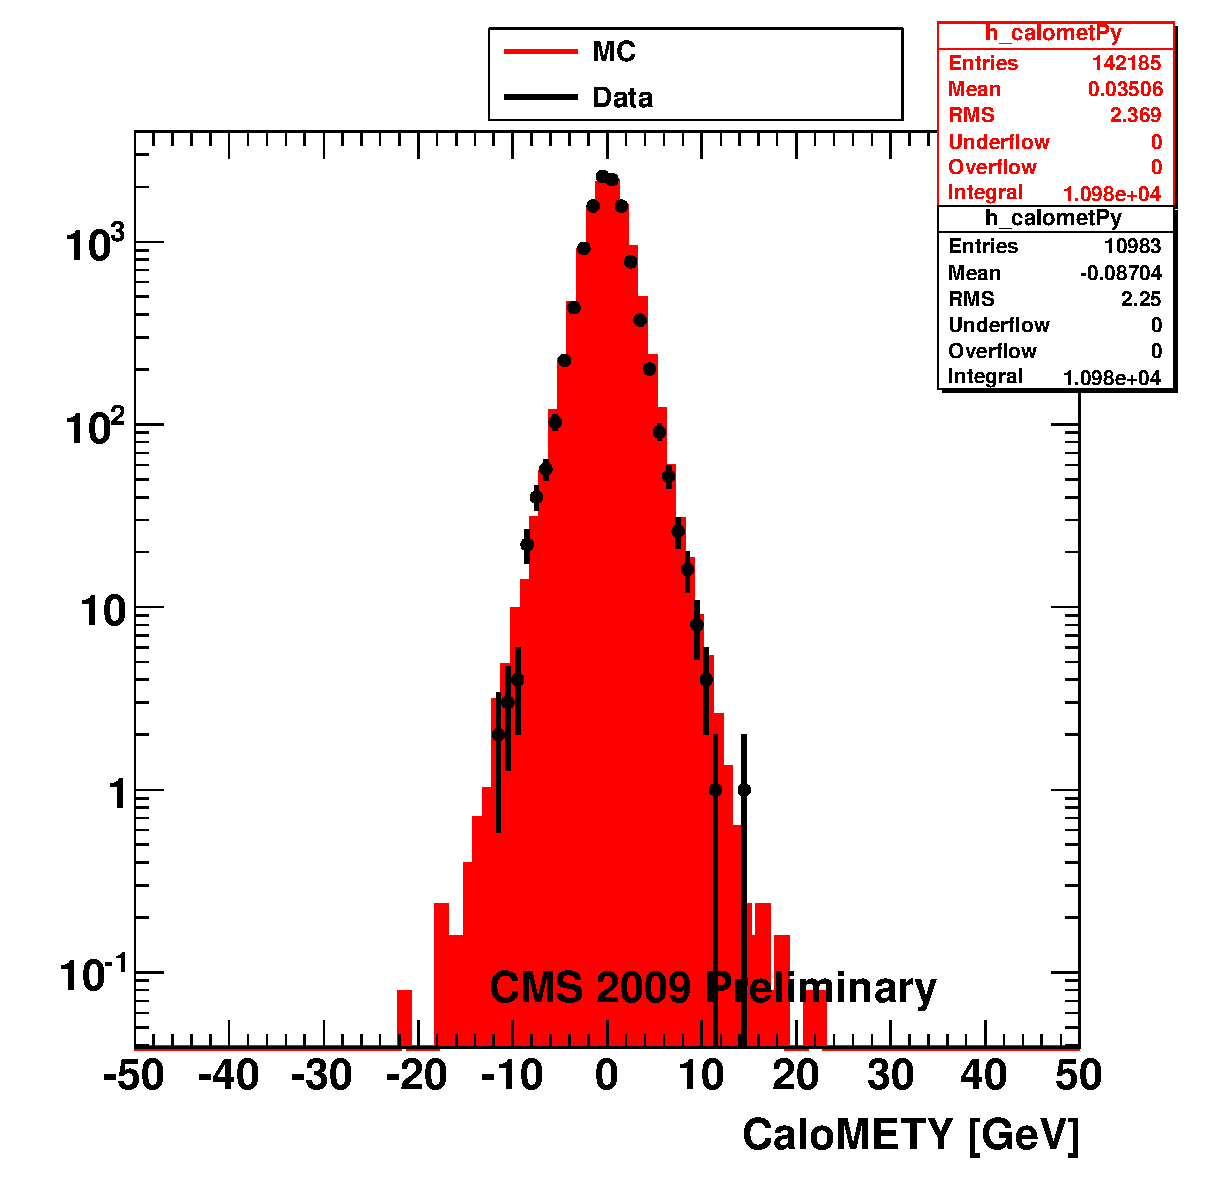
\includegraphics[width=0.40\textwidth]{plots_DataVsMC_MB_2360GeV/h_calometPy.eps} \\
 \end{tabular}
 \caption{$\exmiss$ and $\eymiss$ distributions in 2360 GeV data compared
   with Monte Carlo simulation.
          \label{fig:DataVsMC_MB_2360_2}}
\end{figure}

\begin{figure}[h!]
 \centering
 \begin{tabular}{ll}
  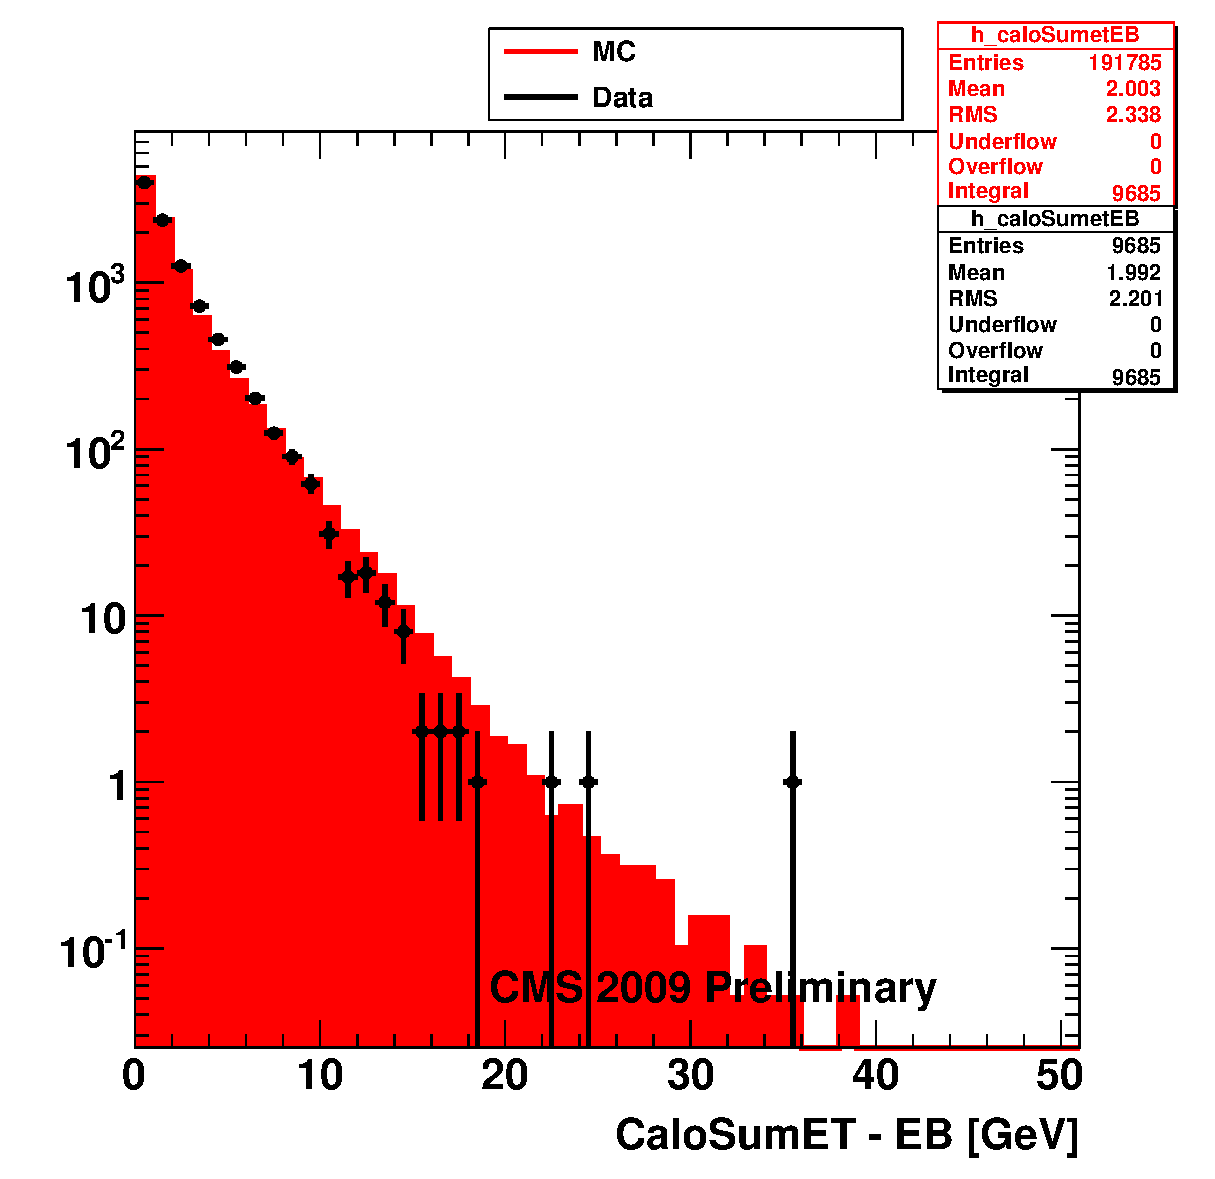
\includegraphics[width=0.40\textwidth]{plots_DataVsMC_MB_2360GeV/h_caloSumetEB.eps} &
  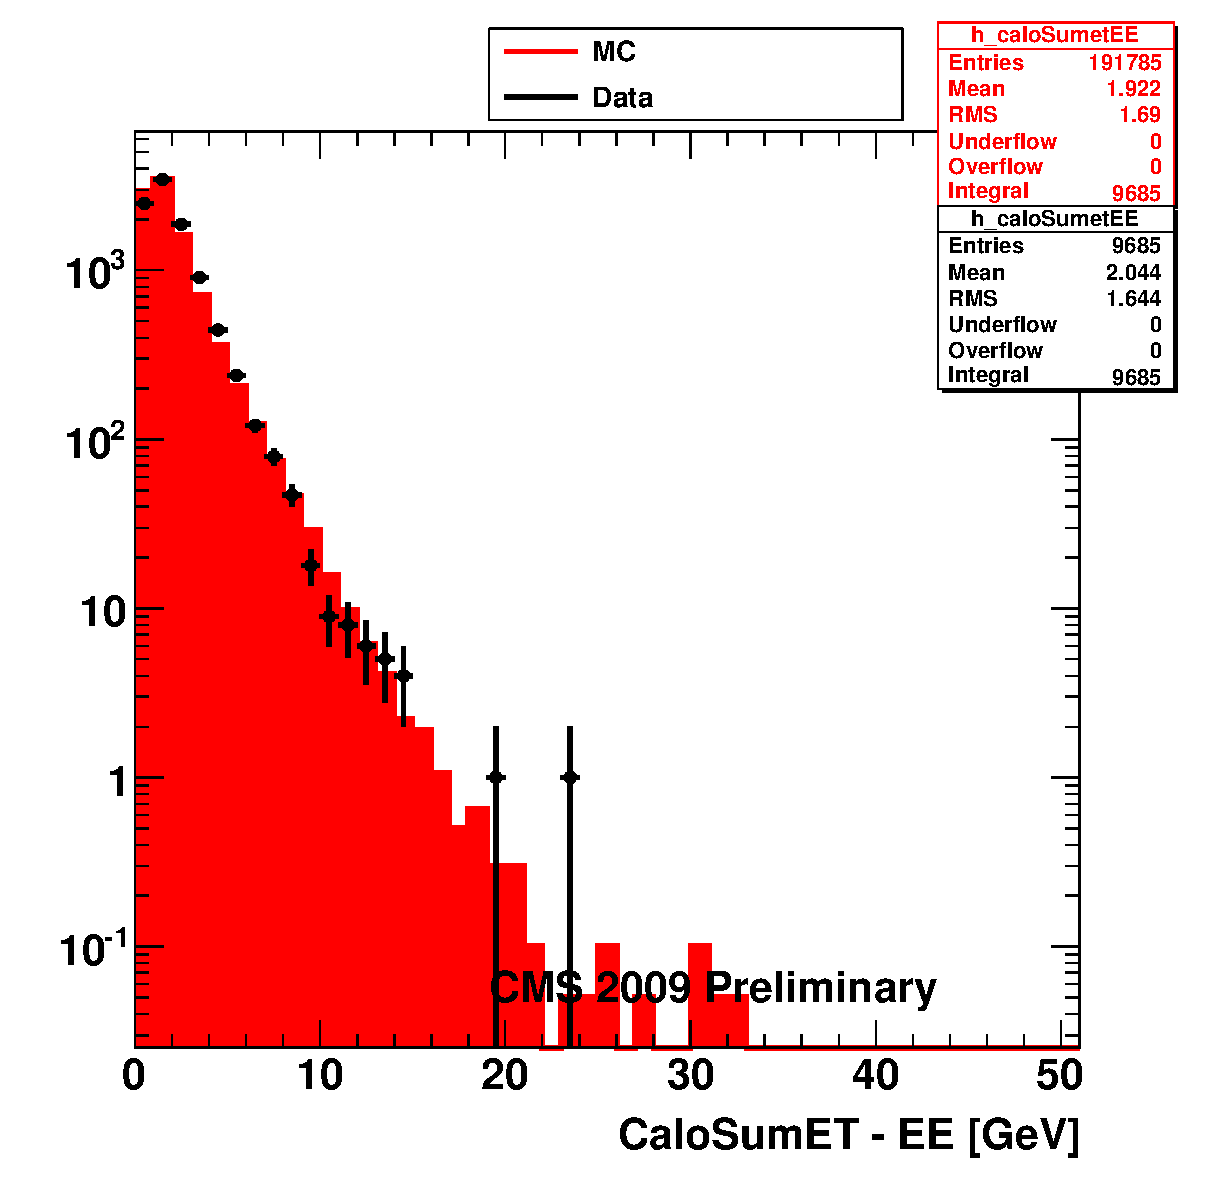
\includegraphics[width=0.40\textwidth]{plots_DataVsMC_MB_2360GeV/h_caloSumetEE.eps} \\
 \end{tabular}
 \caption{$\sumet$ in ECAL barrel and endcap in 2360 GeV data compared
   with Monte Carlo simulation.
          \label{fig:DataVsMC_MB_2360_4}}
\end{figure}

\begin{figure}[h!]
 \centering
 \begin{tabular}{ll}
  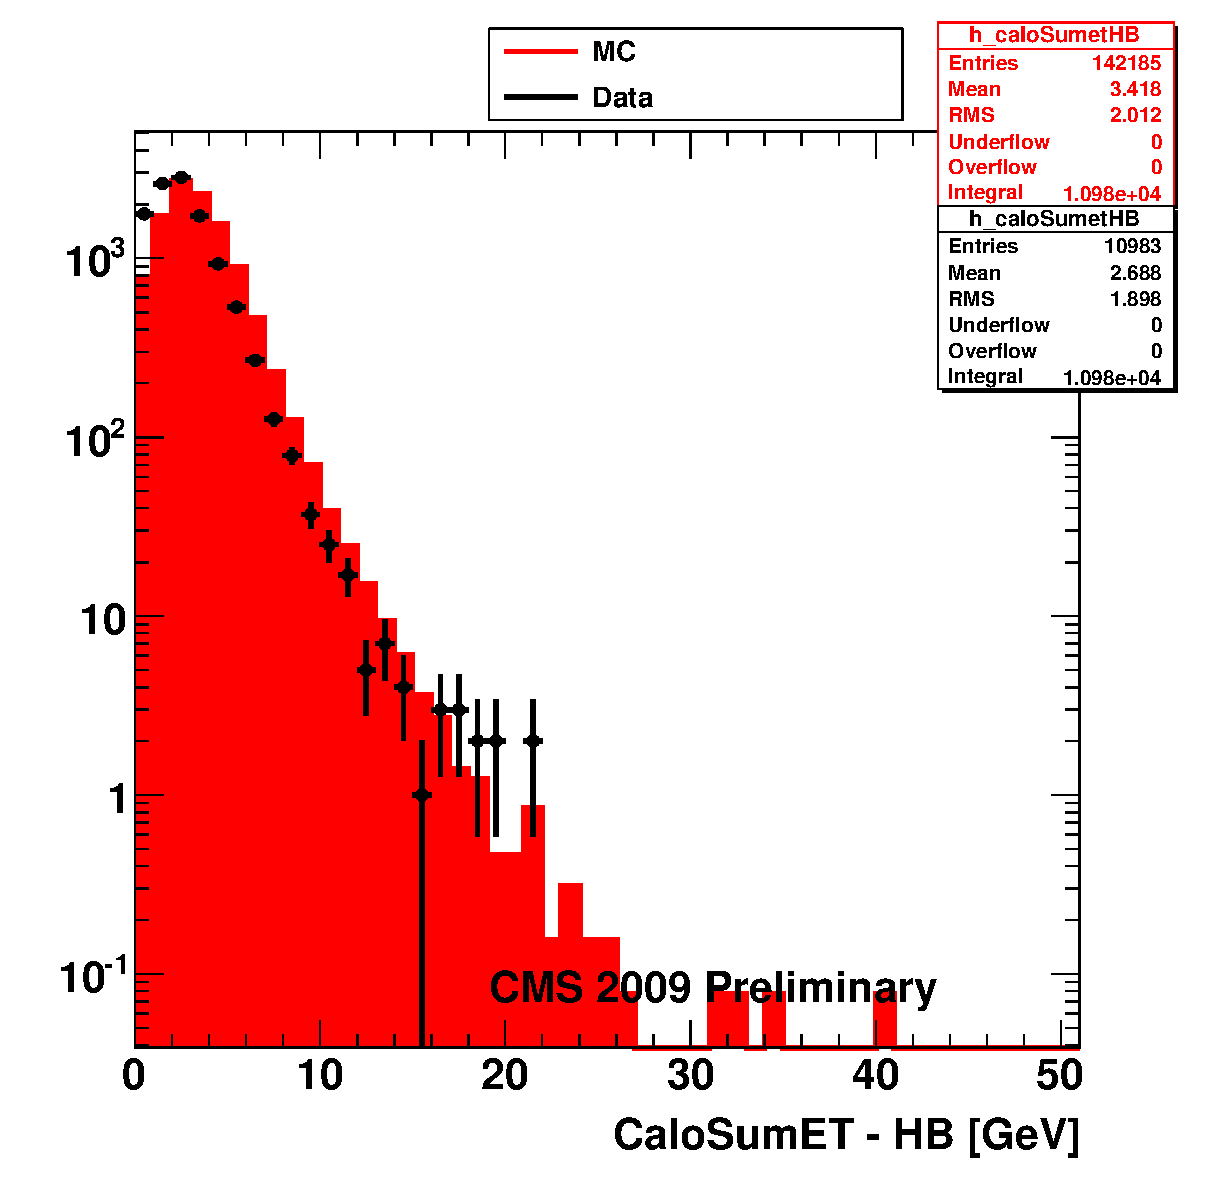
\includegraphics[width=0.40\textwidth]{plots_DataVsMC_MB_2360GeV/h_caloSumetHB.eps} &
  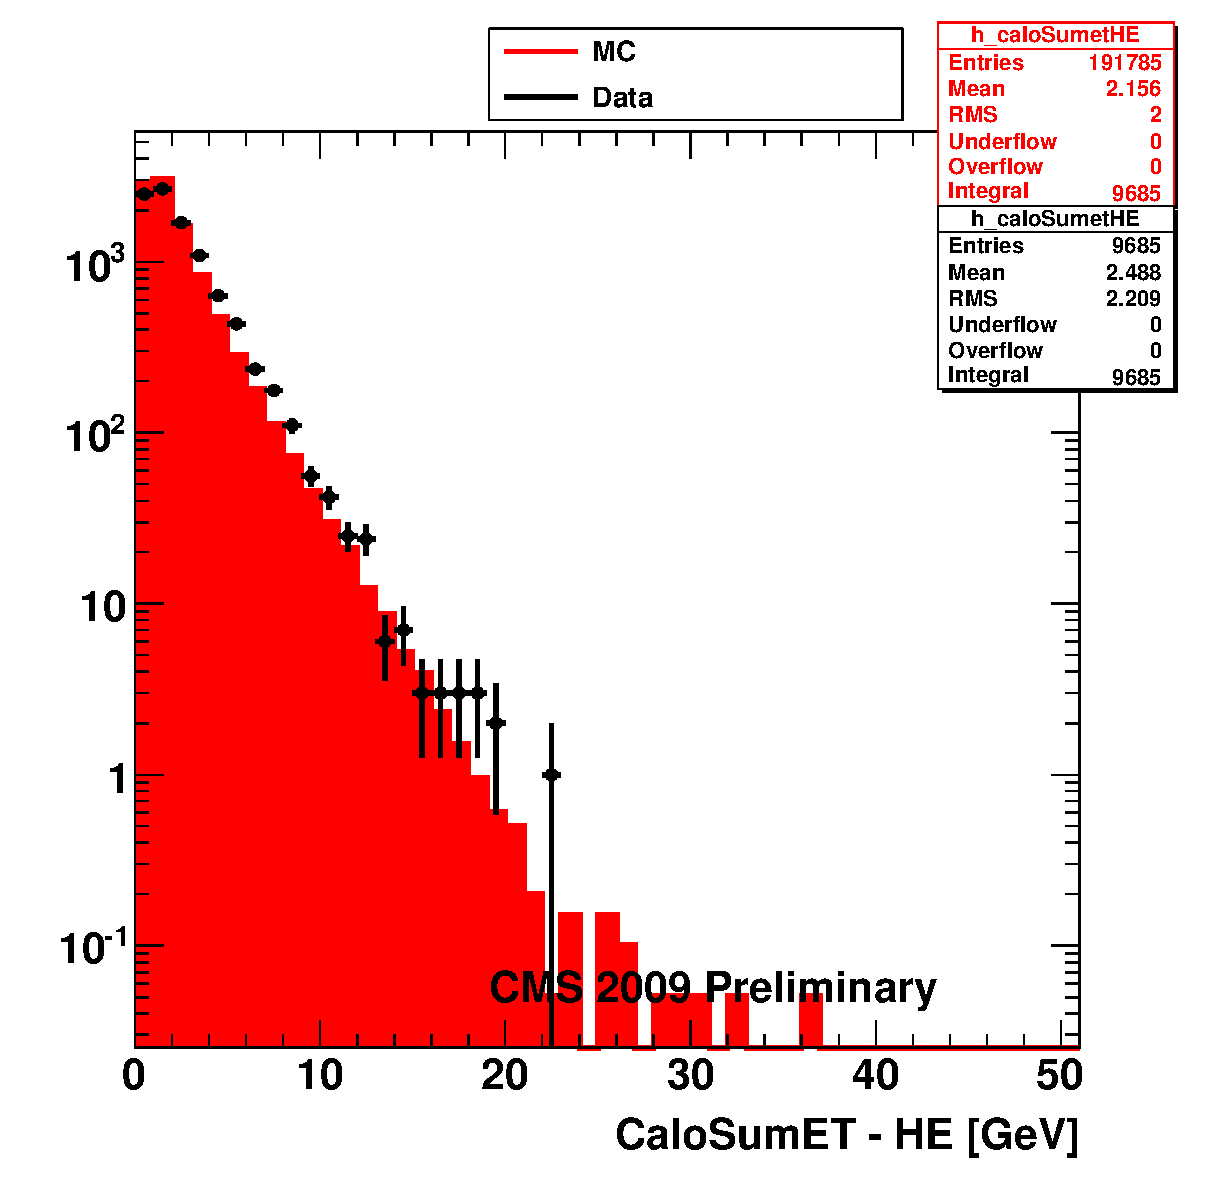
\includegraphics[width=0.40\textwidth]{plots_DataVsMC_MB_2360GeV/h_caloSumetHE.eps} \\
 \end{tabular}
 \caption{$\sumet$ in HCAL barrel and endcap in 2360 GeV data compared
   with Monte Carlo simulation.
          \label{fig:DataVsMC_MB_2360_5}}
\end{figure}

\begin{figure}[h!]
 \centering
 \begin{tabular}{ll}
  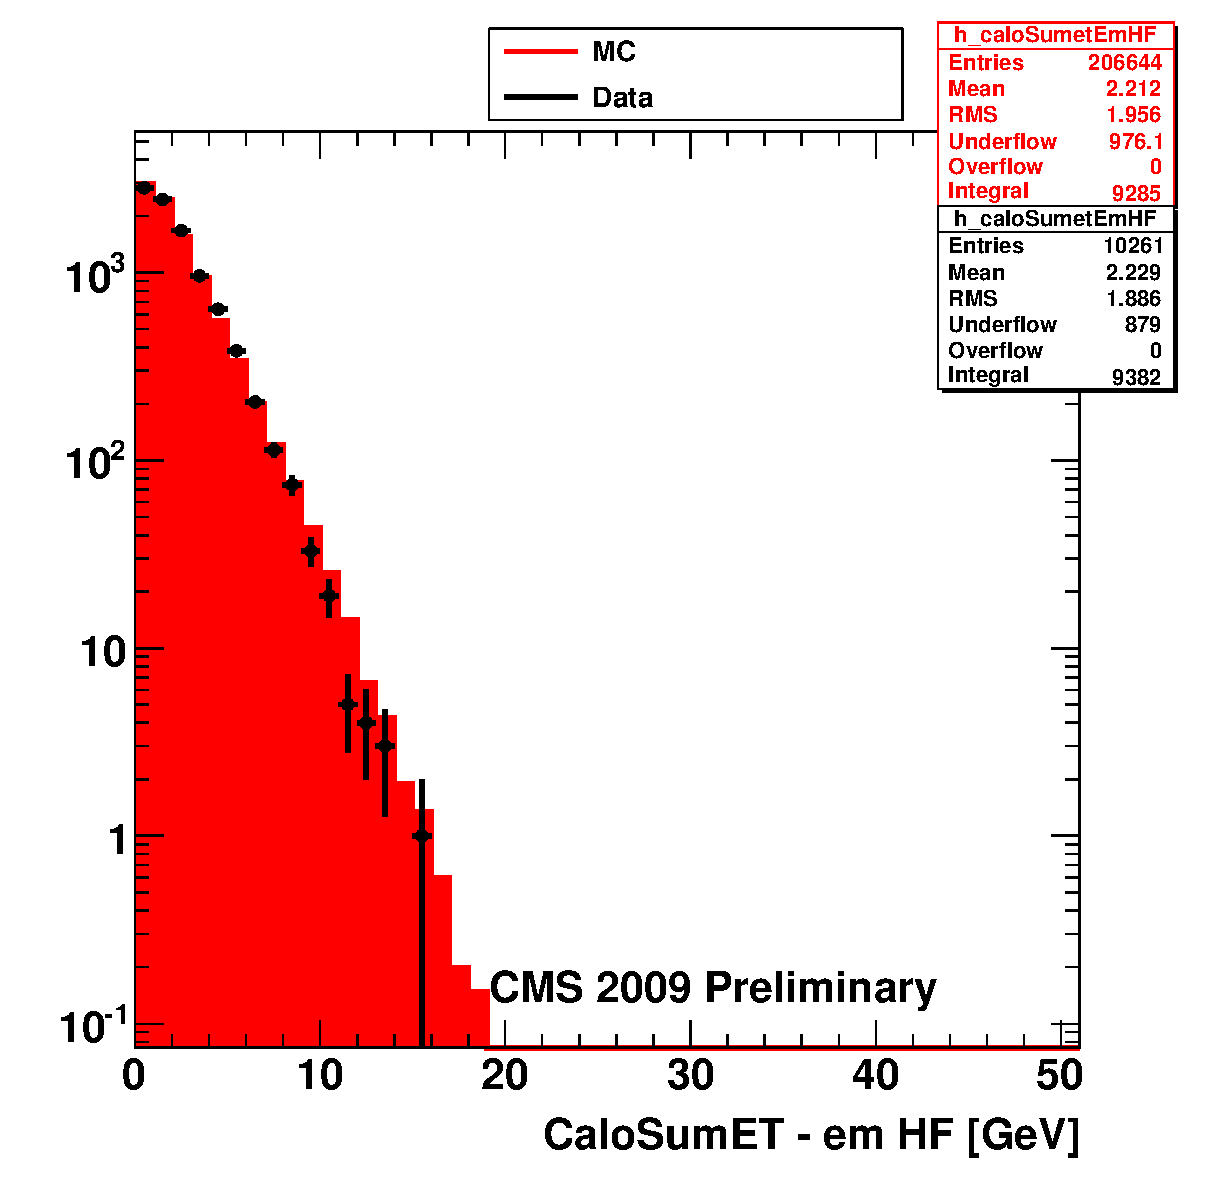
\includegraphics[width=0.40\textwidth]{plots_DataVsMC_MB_2360GeV/h_caloSumetEmHF.eps} &
  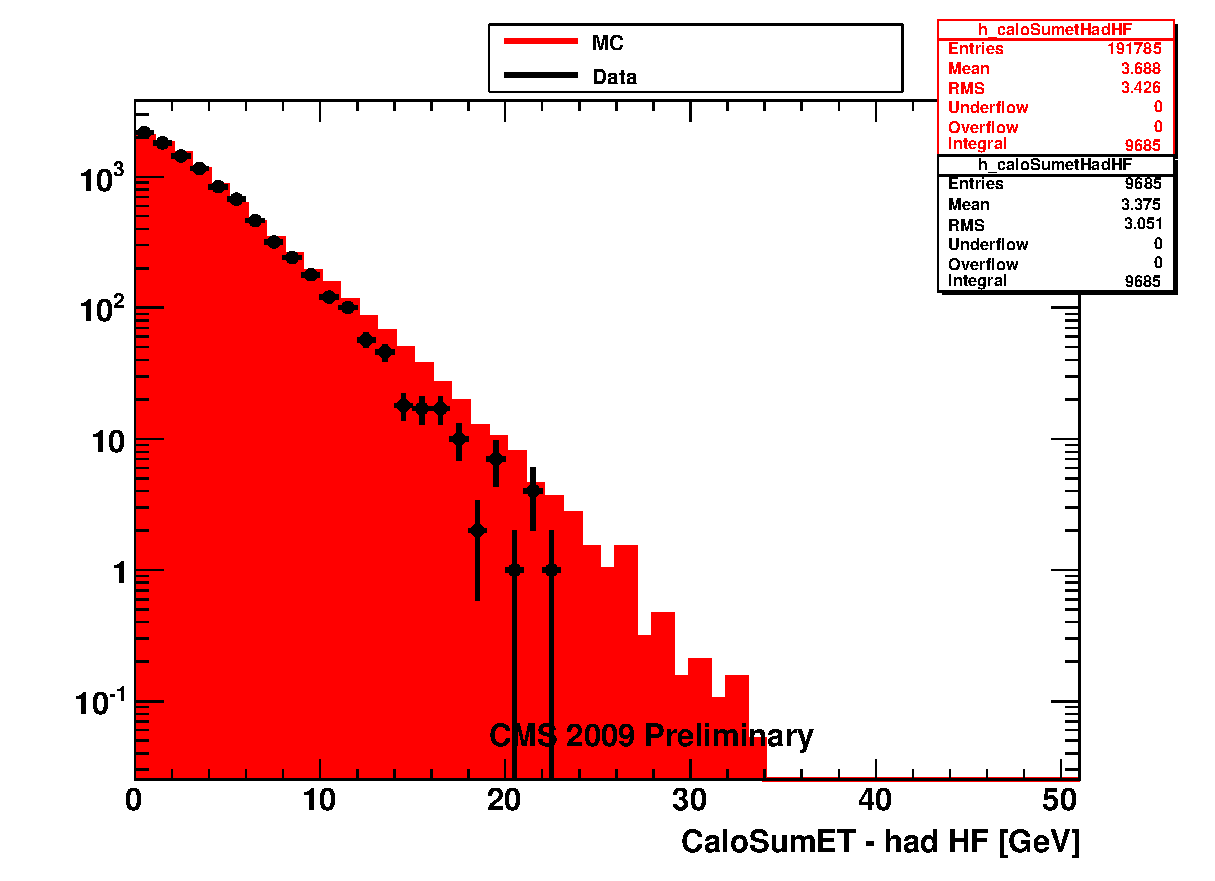
\includegraphics[width=0.40\textwidth]{plots_DataVsMC_MB_2360GeV/h_caloSumetHadHF.eps} \\
 \end{tabular}
 \caption{$\sumet$ in HF in electromagnetic and hadronic parts in 2360 GeV data compared
   with Monte Carlo simulation.
          \label{fig:DataVsMC_MB_2360_6}}

\end{figure}
\begin{figure}[h!]
 \centering
  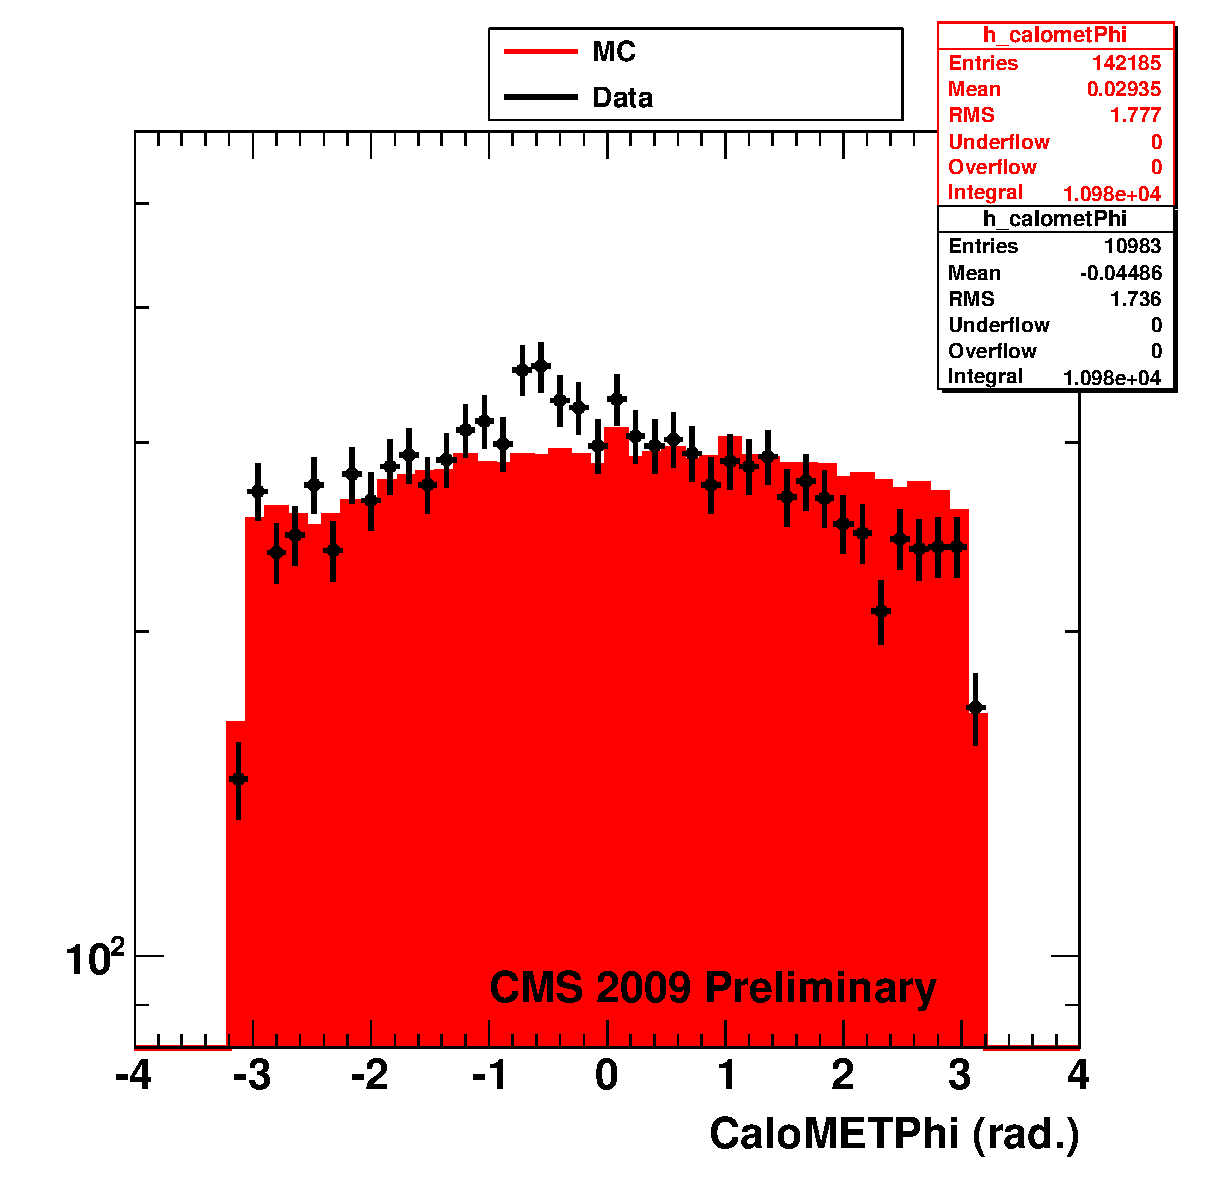
\includegraphics[width=0.40\textwidth]{plots_DataVsMC_MB_2360GeV/h_calometPhi.eps}
 \caption{$\phi_{\etmiss}$ distributions in 2360 GeV data compared
   with Monte Carlo simulation.
          \label{fig:DataVsMC_MB_2360_7}}
\end{figure}

\begin{figure}[h!]
 \centering
 \begin{tabular}{ll}
  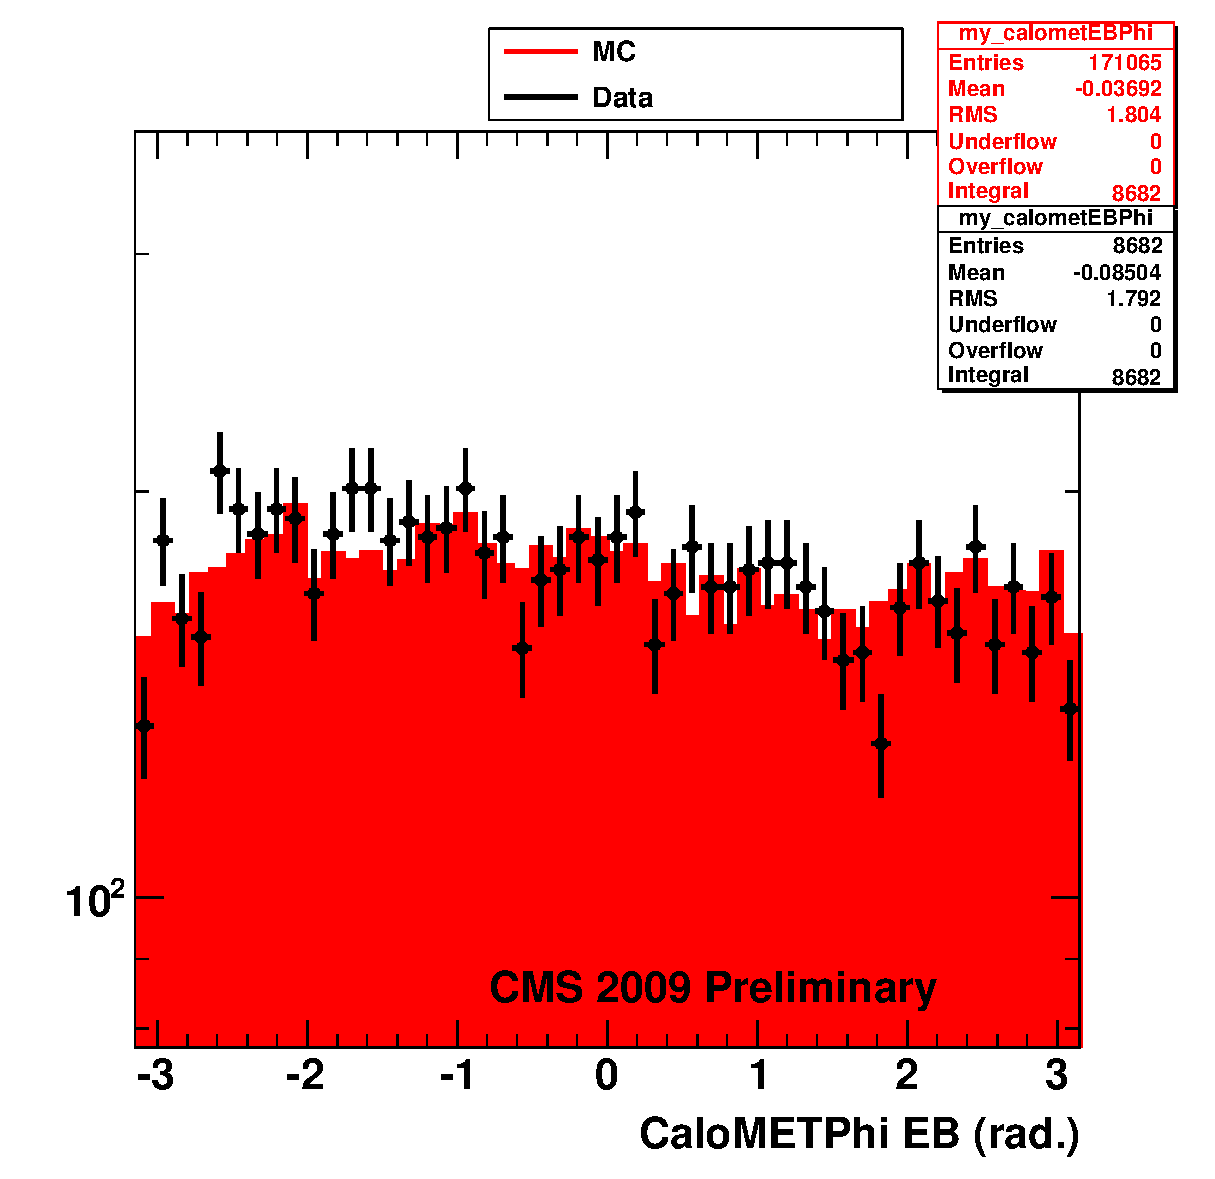
\includegraphics[width=0.40\textwidth]{plots_DataVsMC_MB_2360GeV/my_calometEBPhi.eps} &
  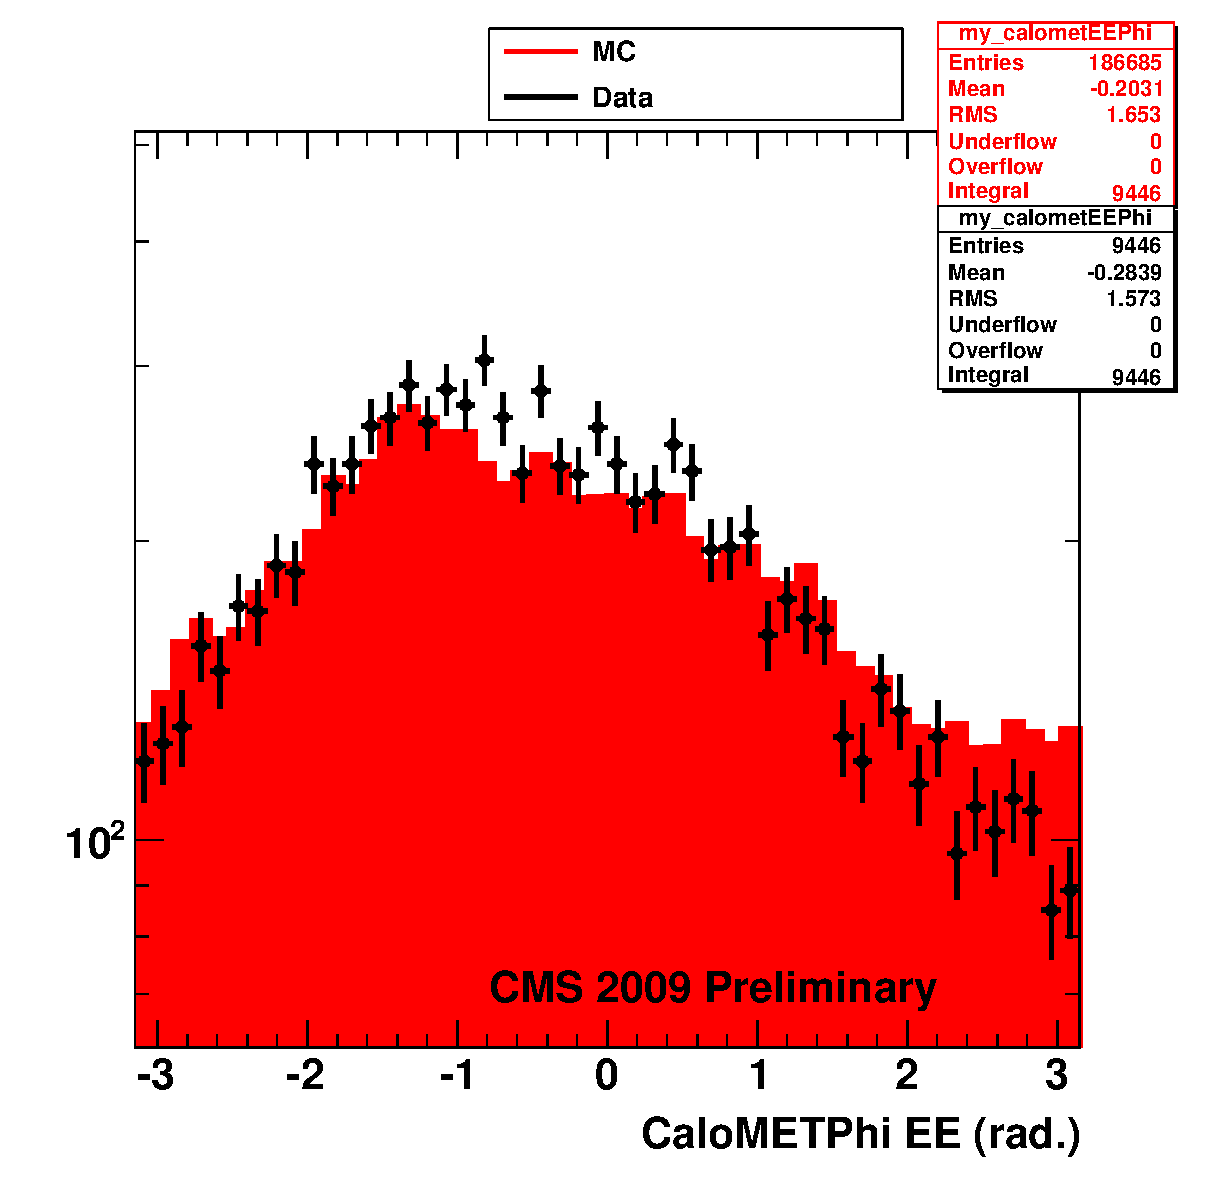
\includegraphics[width=0.40\textwidth]{plots_DataVsMC_MB_2360GeV/my_calometEEPhi.eps} \\
 \end{tabular}
 \caption{$\phi_{\etmiss}$ distributions in ECAL barrel and endcap in 2360 GeV data compared
   with Monte Carlo simulation.
          \label{fig:DataVsMC_MB_2360_8}}
\end{figure}

\begin{figure}[h!]
 \centering
 \begin{tabular}{ll}
  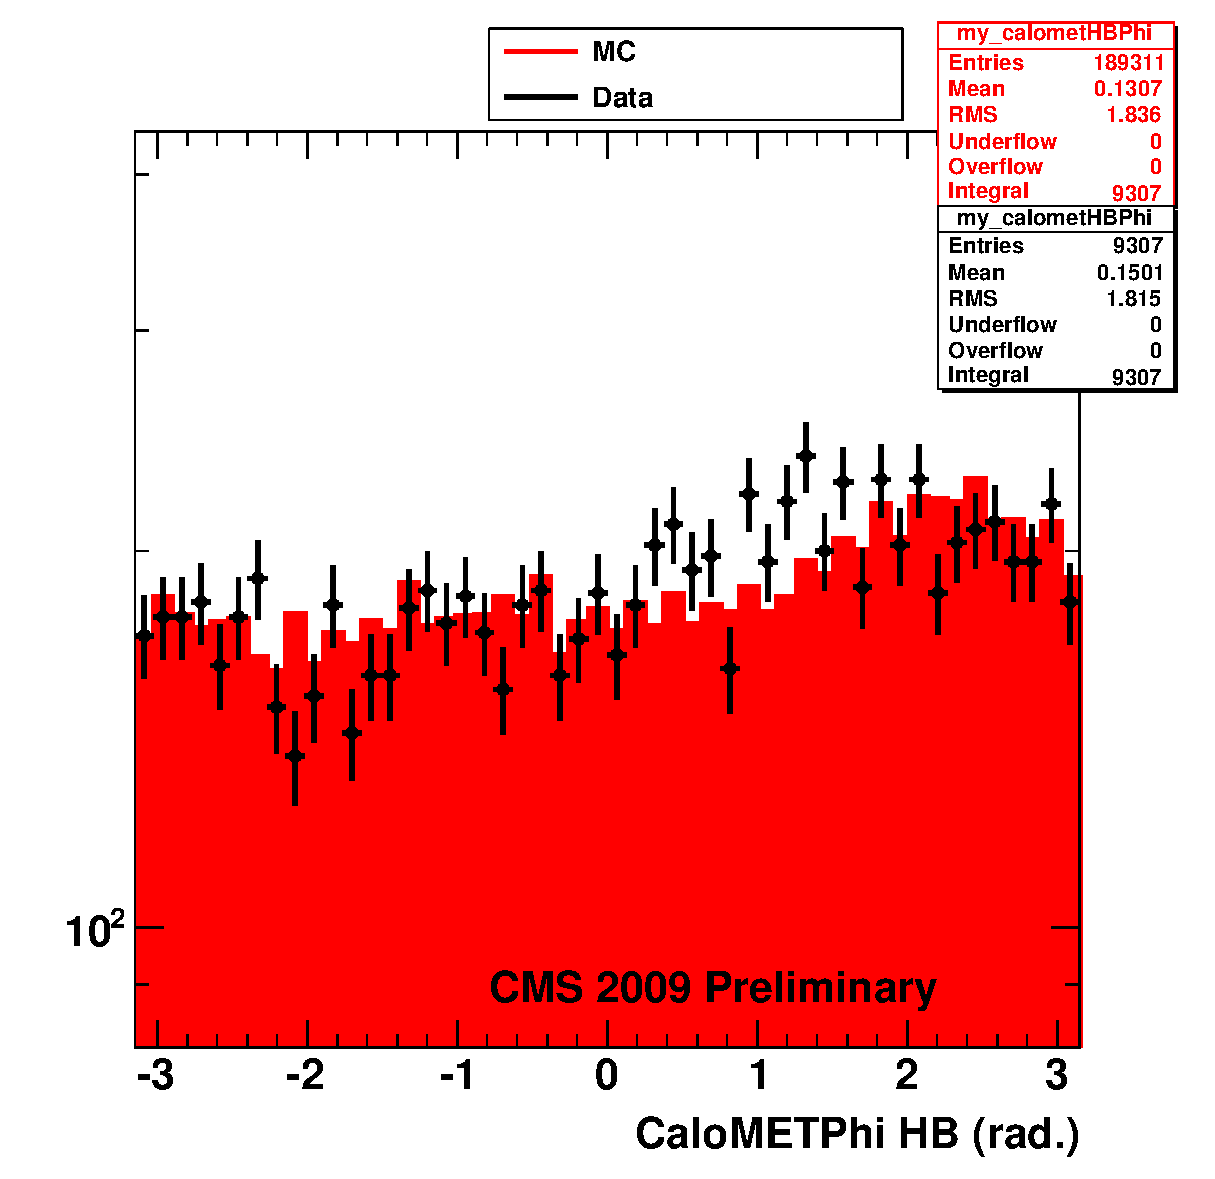
\includegraphics[width=0.40\textwidth]{plots_DataVsMC_MB_2360GeV/my_calometHBPhi.eps} &
  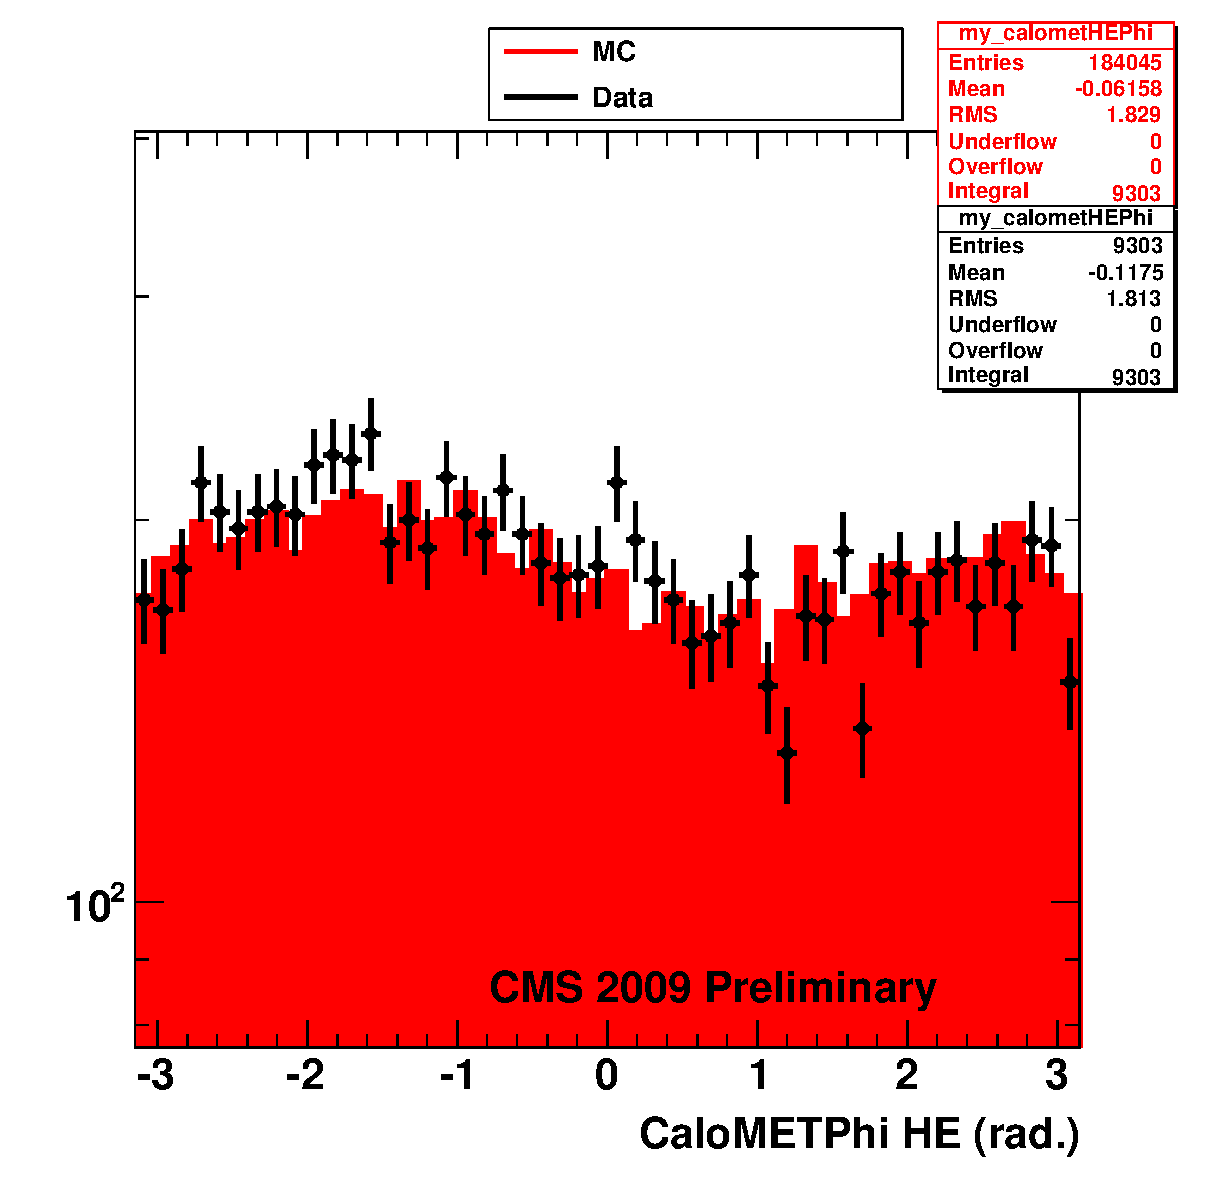
\includegraphics[width=0.40\textwidth]{plots_DataVsMC_MB_2360GeV/my_calometHEPhi.eps} \\
 \end{tabular}
 \caption{$\phi_{\etmiss}$ distributions in HCAL barrel and endcap in 2360 GeV data compared
   with Monte Carlo simulation.
          \label{fig:DataVsMC_MB_2360_9}}
\end{figure}

\begin{figure}[h!]
 \centering
 \begin{tabular}{ll}
  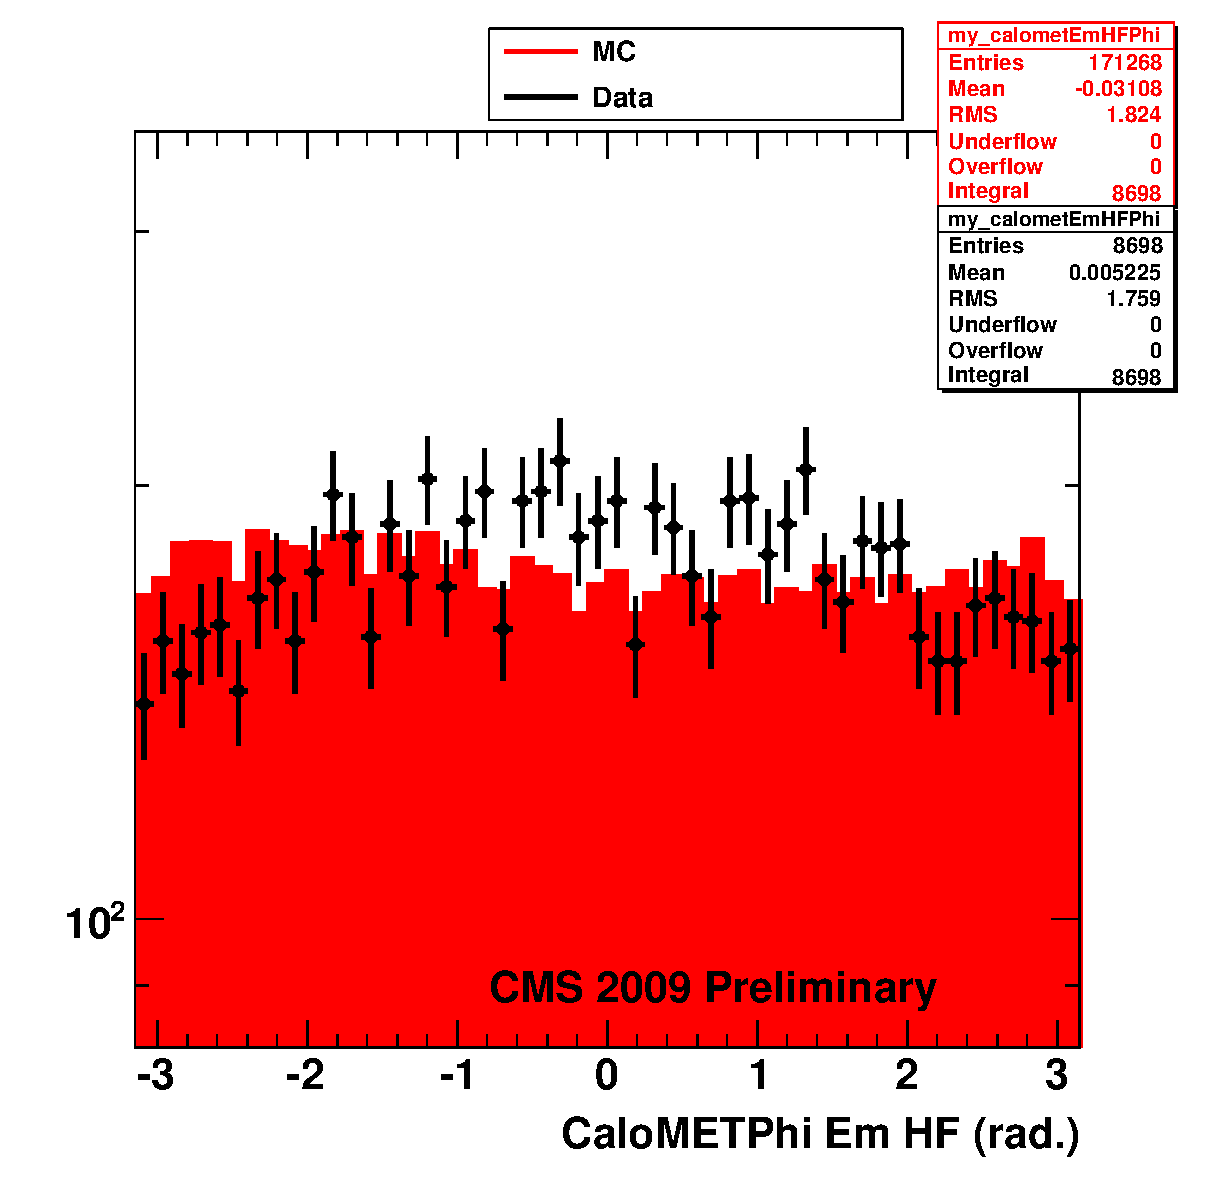
\includegraphics[width=0.40\textwidth]{plots_DataVsMC_MB_2360GeV/my_calometEmHFPhi.eps} &
  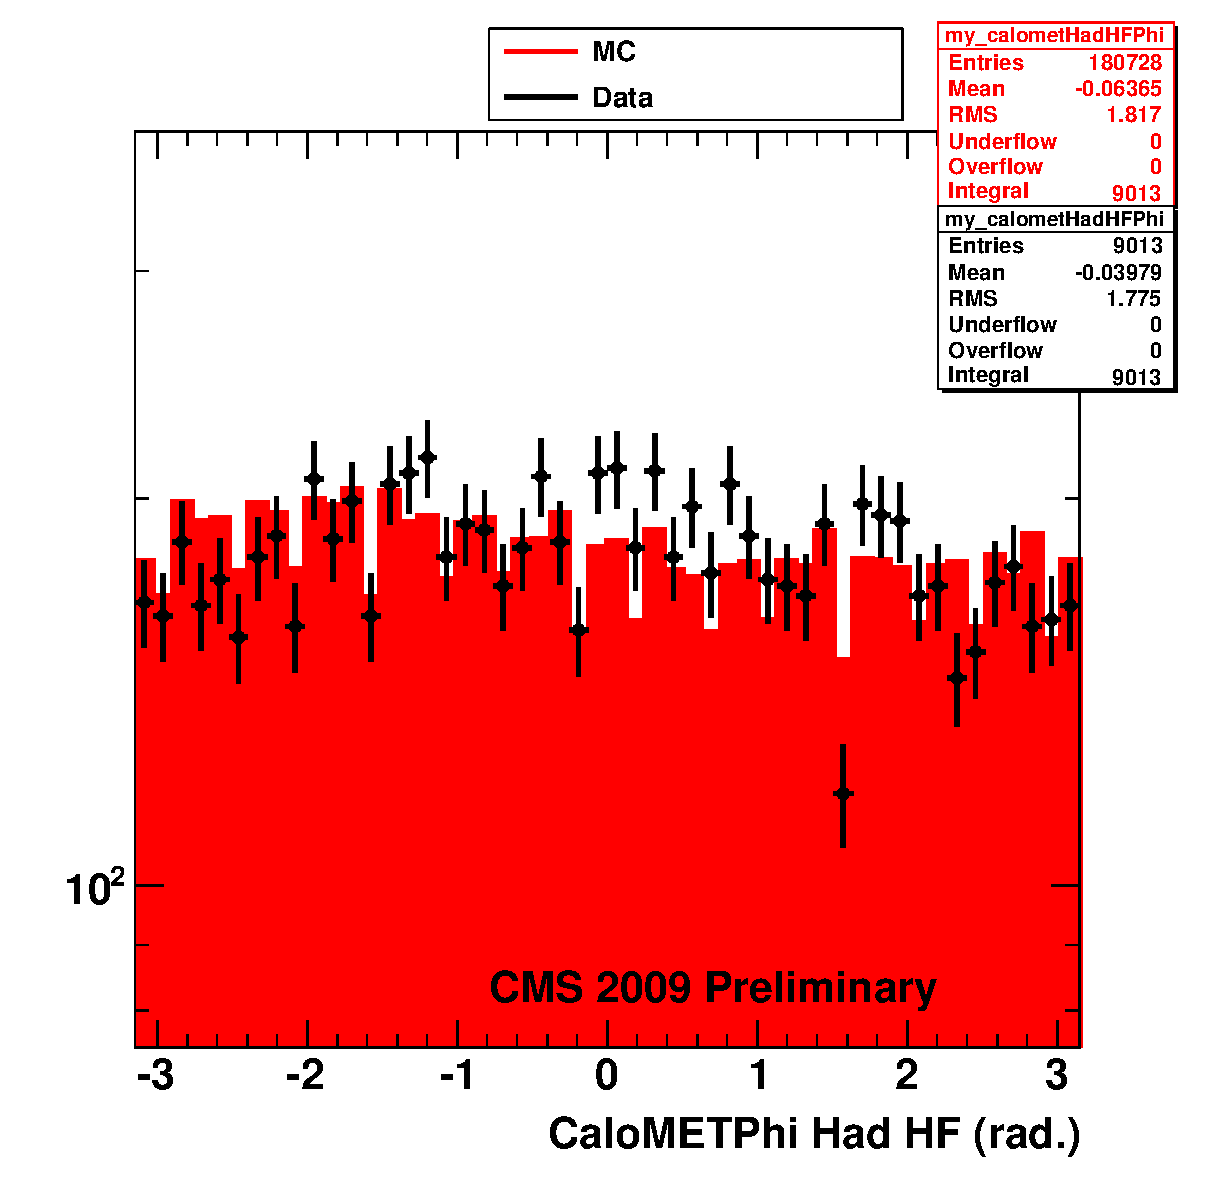
\includegraphics[width=0.40\textwidth]{plots_DataVsMC_MB_2360GeV/my_calometHadHFPhi.eps} \\
 \end{tabular}
 \caption{$\phi_{\etmiss}$ distributions in HF in electromagnetic and hadronic parts in 2360 GeV data compared
   with Monte Carlo simulation.
          \label{fig:DataVsMC_MB_2360_10}}
\end{figure}

\clearpage

\subsection[$\etmiss$ resolution]{$\etmissB$ resolution}

Here we present the same $\etmiss$ resolution analysis as the one presented in Section~\ref{sc:DataVsMCMB900} for the $900$ data. 
Figure~\ref{fig:MExySigma_vs_SumET_2360} shows the $\sigma\left(\exmiss\right)$ and $\sigma\left(\eymiss\right)$ 
vs. $\sum E_\text{T}$ for 2360 GeV data compared with Monte Carlo simulation. Figures~\ref{fig:MExSigma_vs_SumET_2360_fit} 
and \ref{fig:MEySigma_vs_SumET_2360_fit} show the fit of $\sigma\left(\exmiss\right)$ and $\sigma\left(\eymiss\right)$ vs. 
$\sum E_\text{T}$ to Eq.~\ref{eq:MET_sigma} for data and  Monte Carlo at $2360$ GeV.

\begin{figure}[h!]
 \centering
 \begin{tabular}{ll}
  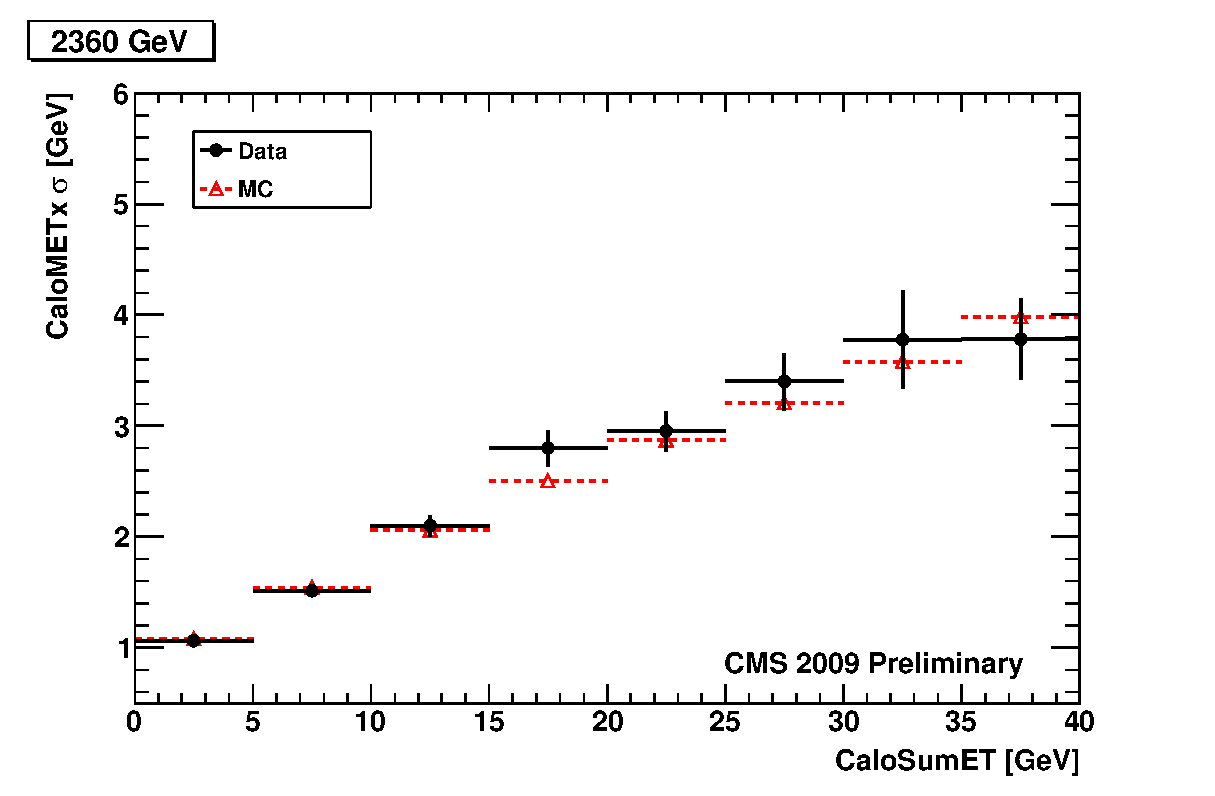
\includegraphics[width=0.5\textwidth]{plots_DataVsMC_MB_2360GeV/h_metxsigma_sumet_2360.eps} &
  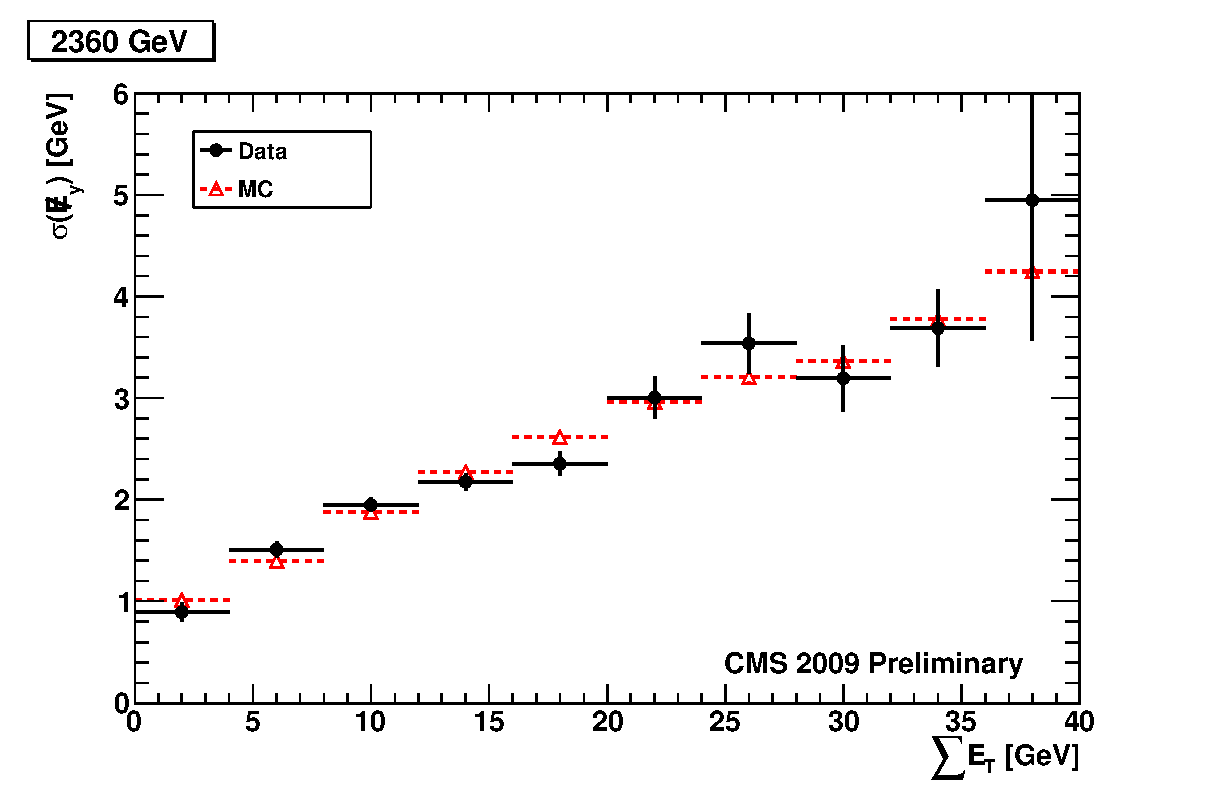
\includegraphics[width=0.5\textwidth]{plots_DataVsMC_MB_2360GeV/h_metysigma_sumet_2360.eps} \\
 \end{tabular}
 \caption{\small $\sigma\left(\exmiss\right)$ and $\sigma\left(\eymiss\right)$ $\sigma$ vs. $\sum E_\text{T}$ for
          data at $2360$ TeV compared with Monte Carlo simulation.\label{fig:MExySigma_vs_SumET_2360}}
\end{figure}

\begin{figure}[h!]
 \centering
 \begin{tabular}{ll}
  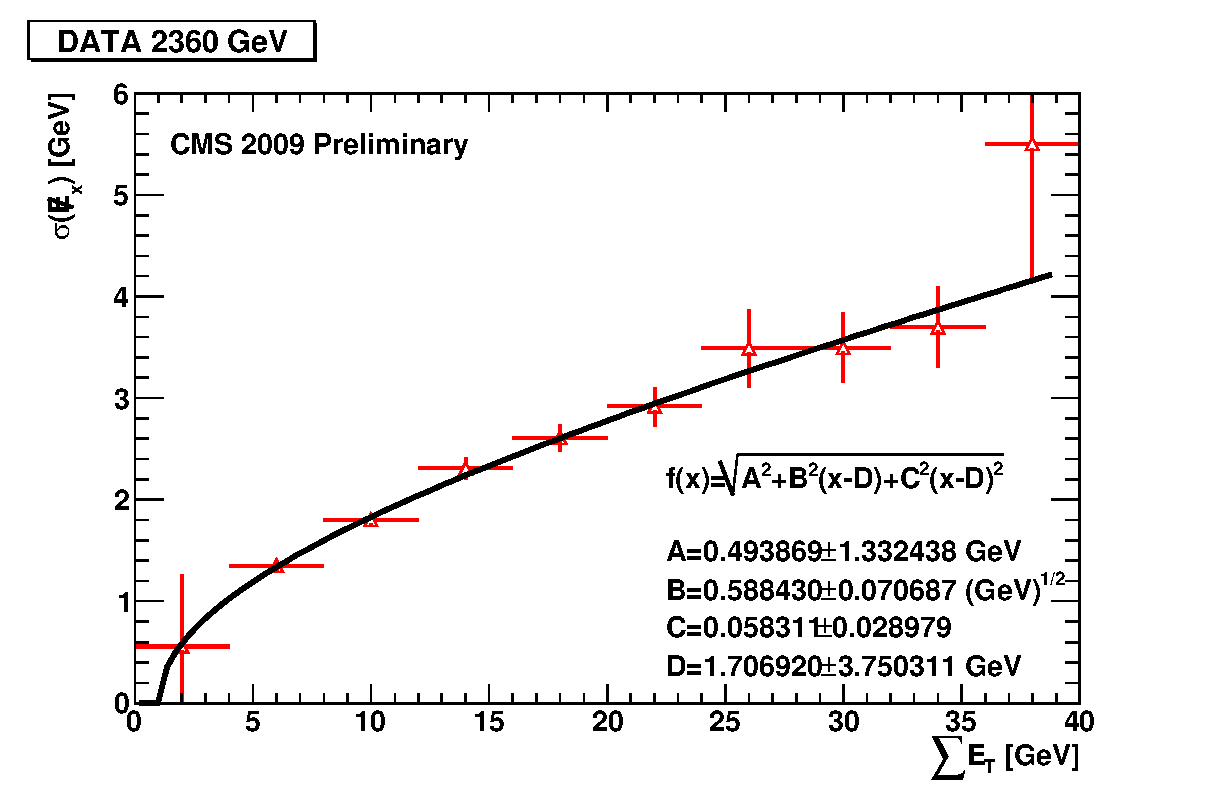
\includegraphics[width=0.5\textwidth]{plots_DataVsMC_MB_2360GeV/final_metxsigma_sumet_DATA_2360.eps} &
  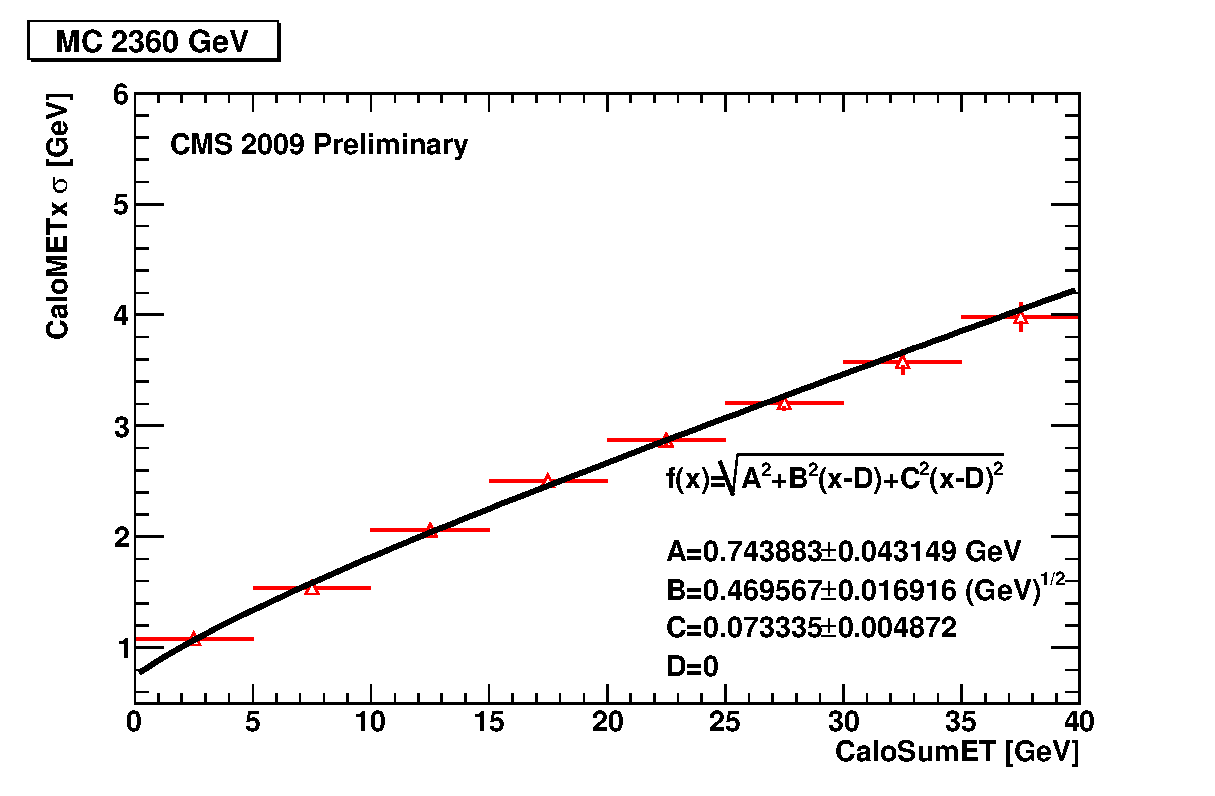
\includegraphics[width=0.5\textwidth]{plots_DataVsMC_MB_2360GeV/final_metxsigma_sumet_MC_2360.eps} \\
 \end{tabular}
 \caption{\small Fit of the $\sigma\left(\exmiss\right)$ vs. $\sum E_\text{T}$ for data and Monte Carlo at $2360$ GeV.\label{fig:MExSigma_vs_SumET_2360_fit}}
\end{figure}

\begin{figure}[h!]
 \centering
 \begin{tabular}{ll}
  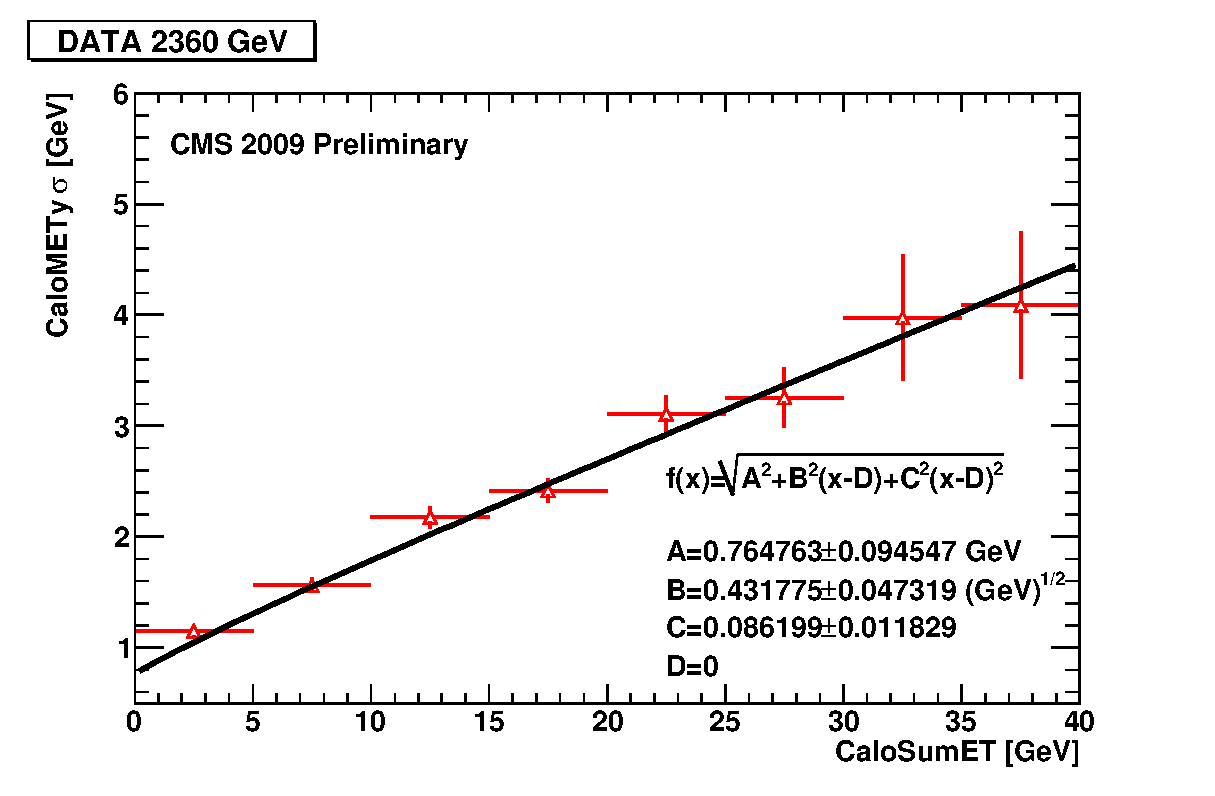
\includegraphics[width=0.5\textwidth]{plots_DataVsMC_MB_2360GeV/final_metysigma_sumet_DATA_2360.eps} &
  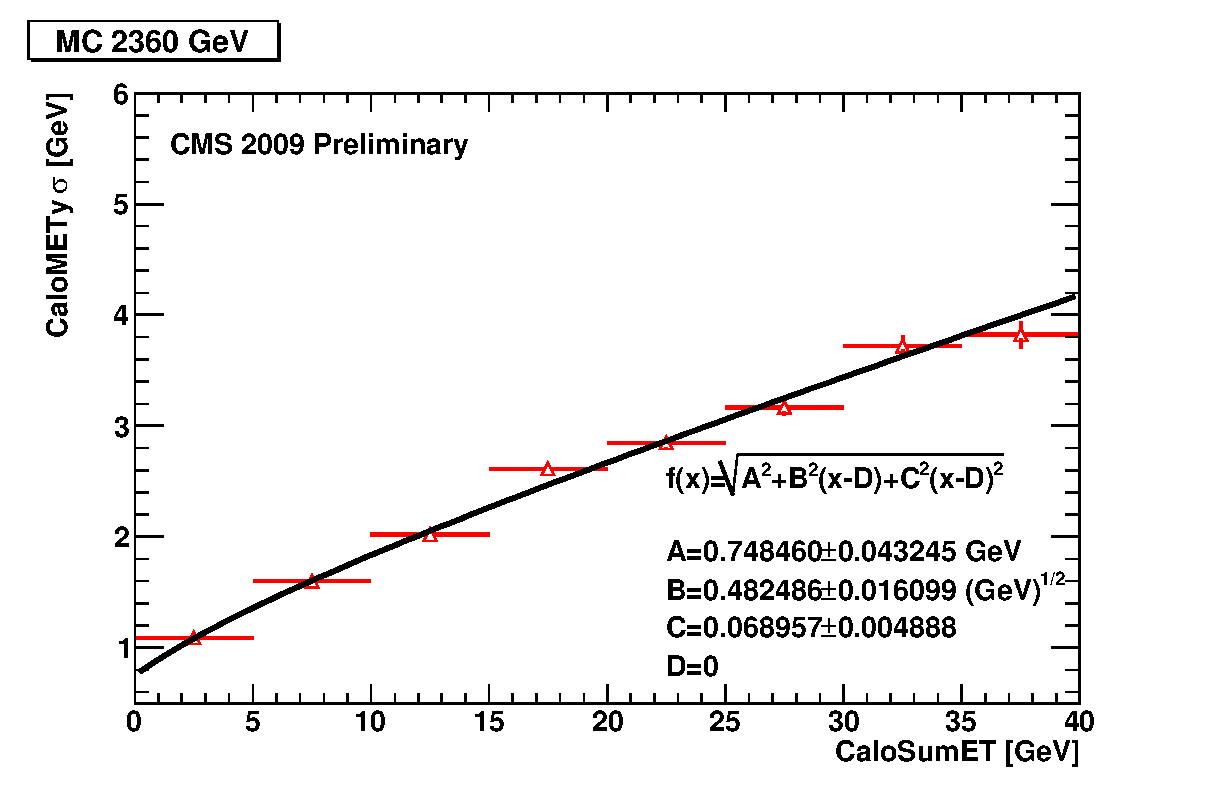
\includegraphics[width=0.5\textwidth]{plots_DataVsMC_MB_2360GeV/final_metysigma_sumet_MC_2360.eps} \\
 \end{tabular}
 \caption{\small Fit of the $\sigma\left(\eymiss\right)$ vs. $\sum E_\text{T}$ for data and Monte Carlo at $2360$ GeV.\label{fig:MEySigma_vs_SumET_2360_fit}}
\end{figure}

\clearpage

\subsection[$\etmiss$ and $\sumet$ dependence on $\eta$]{$\etmissB$ and $\sumetB$ dependence on $\boldsymbol{\eta}$} \label{sec:MetVarVsIeta_2360}

\begin{figure}[h!]
 \centering
 \begin{tabular}{ll}
  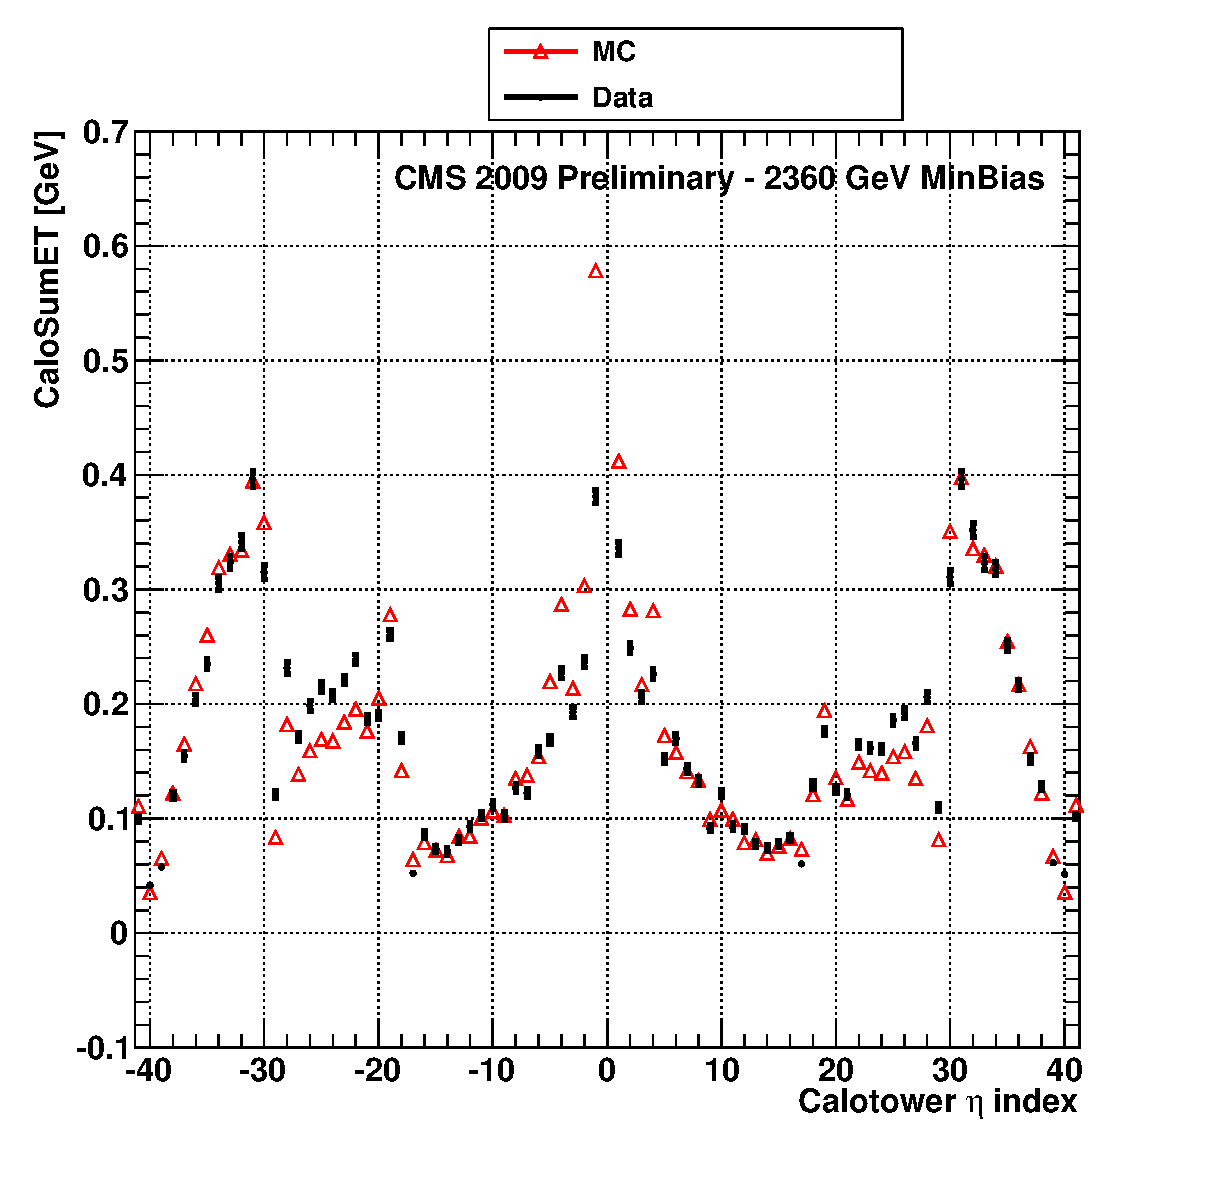
\includegraphics[width=0.5\textwidth]{plots_DataVsMC_MB_2360GeV/g_caloSumetMean_vs_ieta_2360.eps} &
  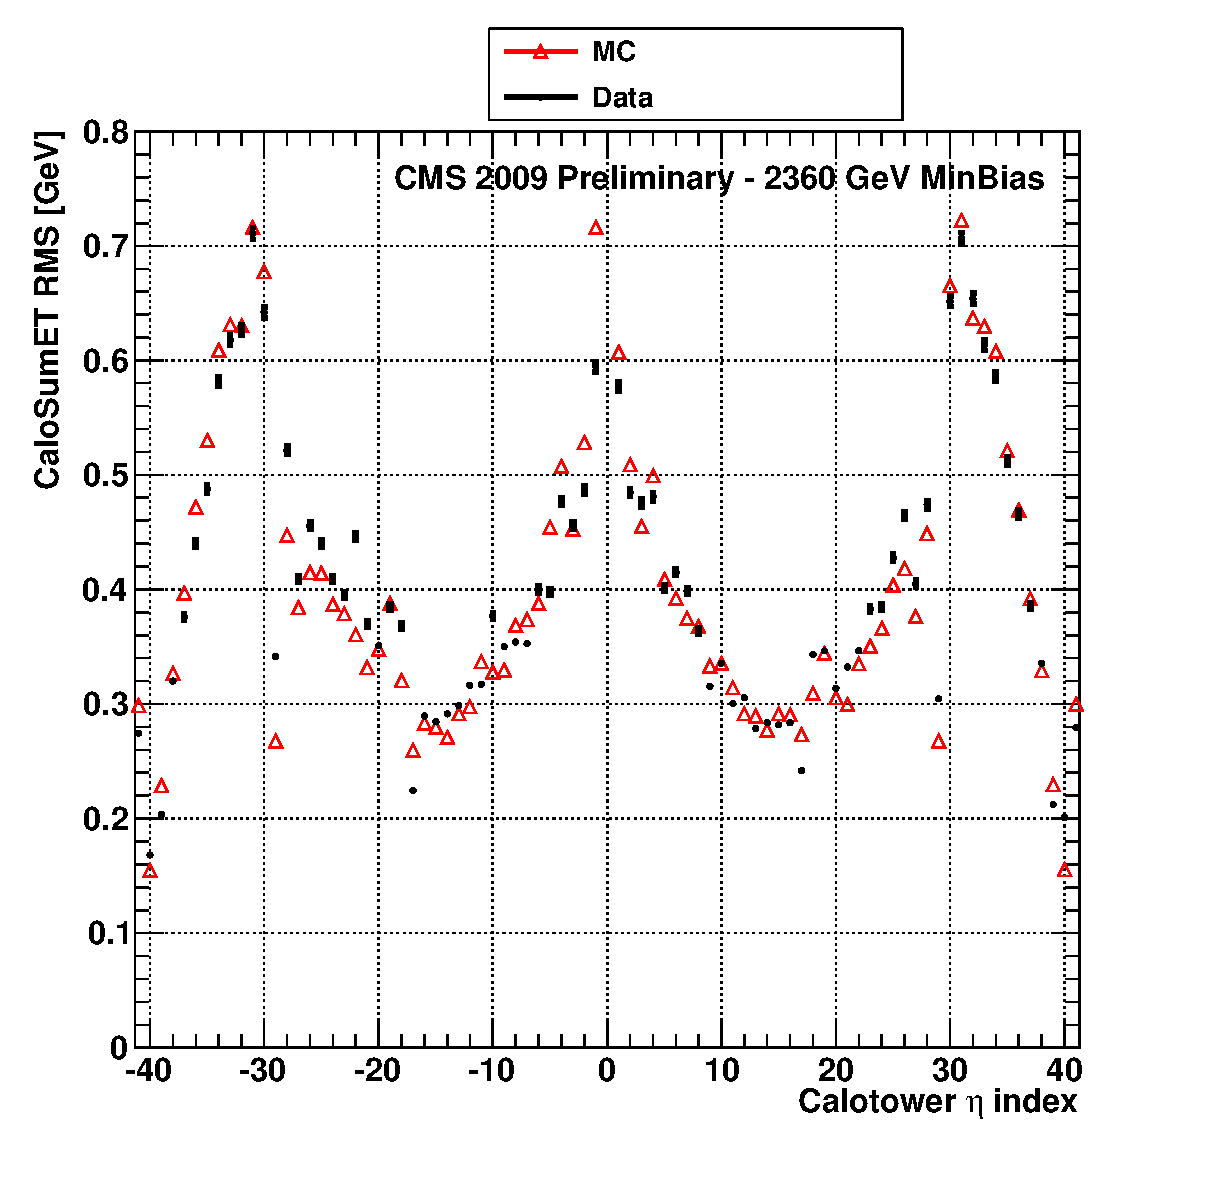
\includegraphics[width=0.5\textwidth]{plots_DataVsMC_MB_2360GeV/g_caloSumetRMS_vs_ieta_2360.eps} \\
 \end{tabular}
 \caption{\small Comparison of the $\sumet$ Mean vs. $i\eta$ of calotowers and $\sumet$ RMS vs. $i\eta$ of calotowers between 
          data and Monte Carlo at $2360$ GeV.\label{fig:SumET_MeanRMS_vs_ieta_2360}}
\end{figure}

\begin{figure}[h!]
 \centering
 \begin{tabular}{ll}
  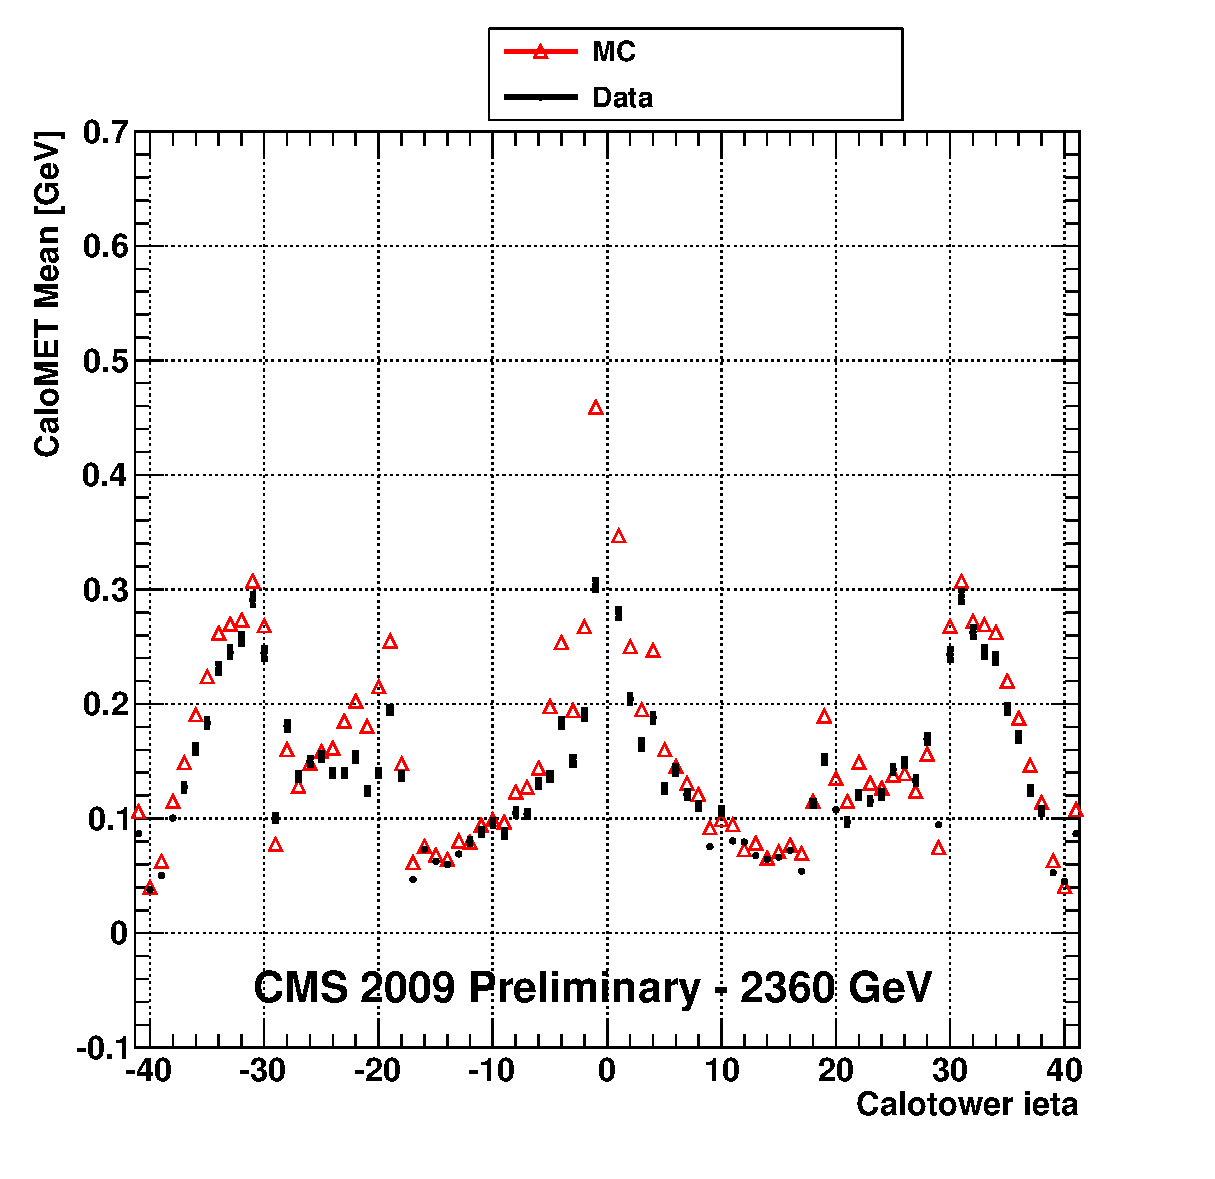
\includegraphics[width=0.5\textwidth]{plots_DataVsMC_MB_2360GeV/g_calometPtMean_vs_ieta_2360.eps} &
  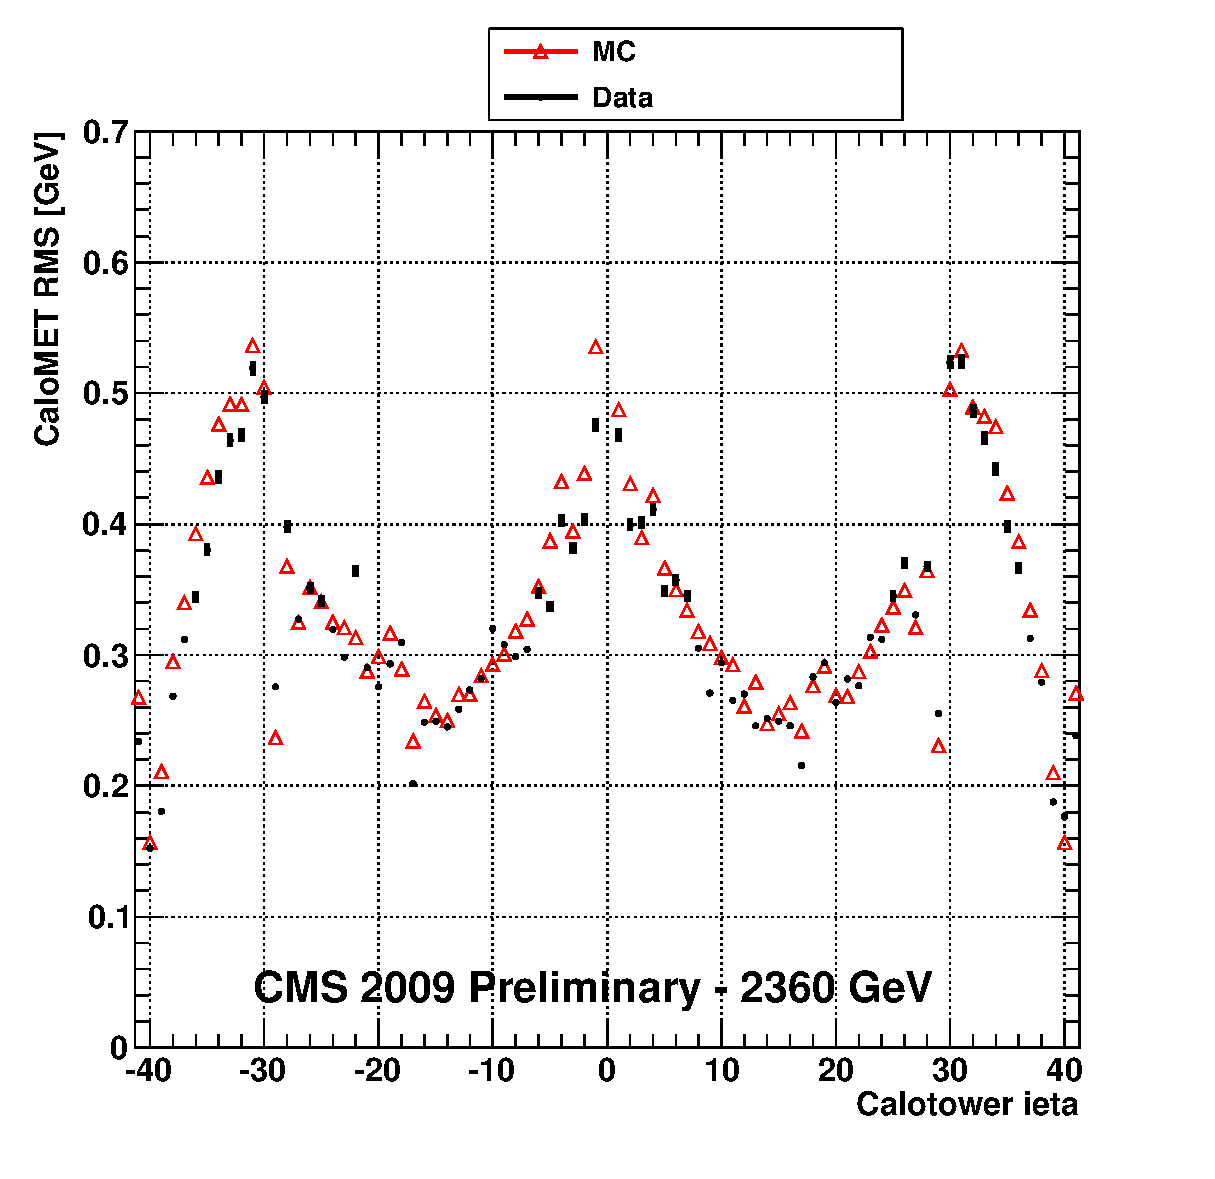
\includegraphics[width=0.5\textwidth]{plots_DataVsMC_MB_2360GeV/g_calometPtRMS_vs_ieta_2360.eps} \\
 \end{tabular}
 \caption{\small Comparison of the $\etmiss$ Mean vs. $i\eta$ of calotowers and $\etmiss$ RMS vs. $i\eta$ of calotowers between 
          data and Monte Carlo at $2360$ GeV.\label{fig:MET_MeanRMS_vs_ieta_2360}}
\end{figure}

\begin{figure}[h!]
 \centering
 \begin{tabular}{ll}
  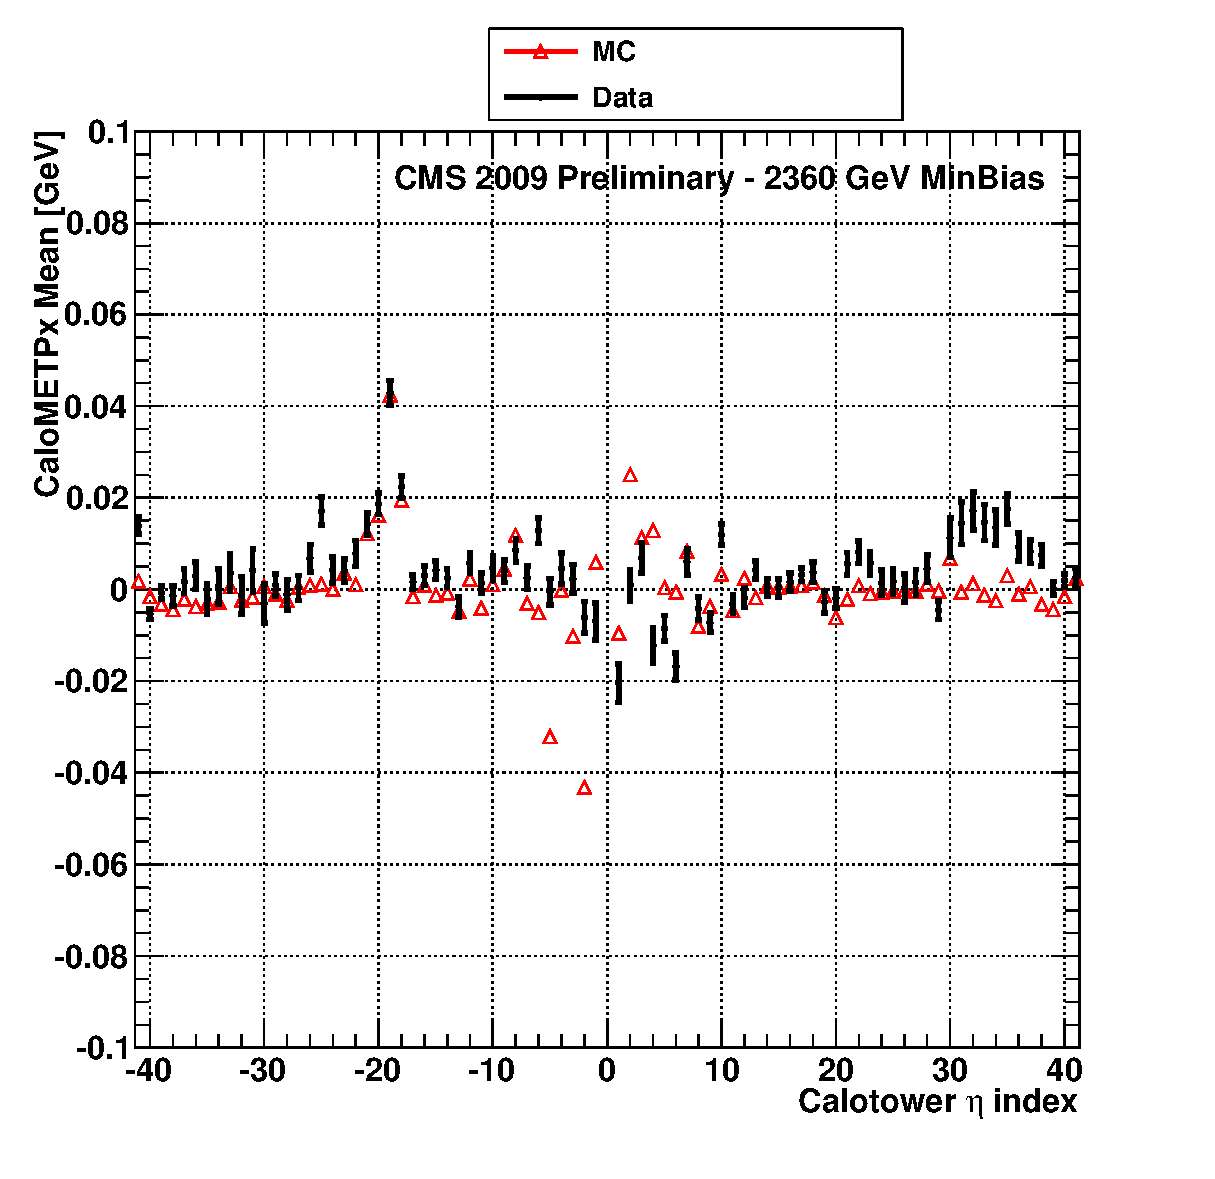
\includegraphics[width=0.5\textwidth]{plots_DataVsMC_MB_2360GeV/g_calometPxMean_vs_ieta_2360.eps} &
  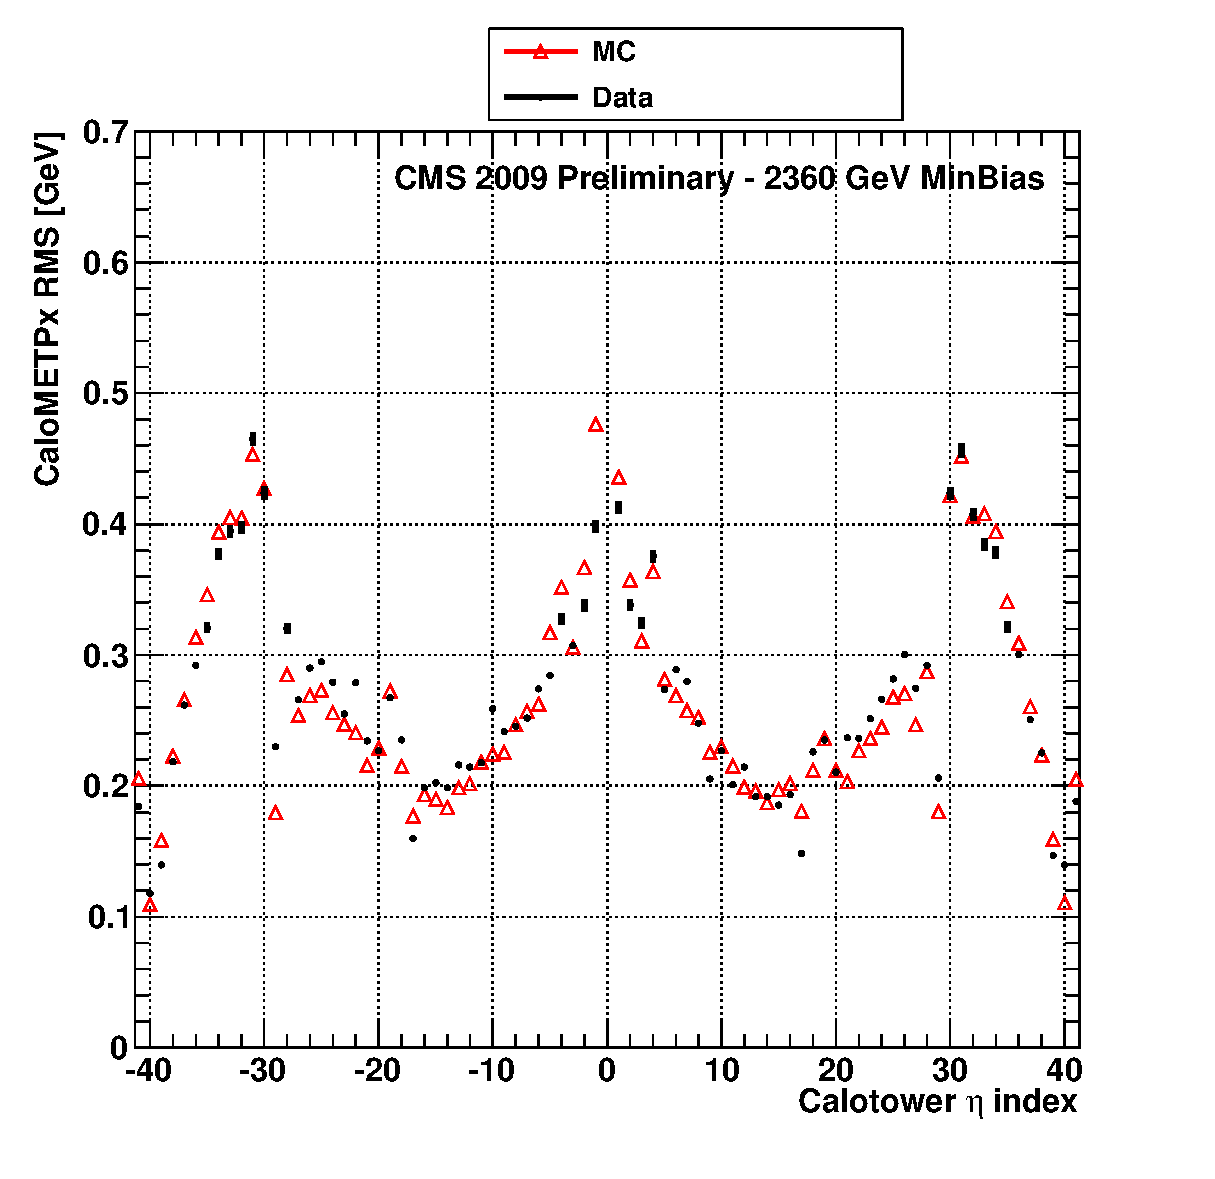
\includegraphics[width=0.5\textwidth]{plots_DataVsMC_MB_2360GeV/g_calometPxRMS_vs_ieta_2360.eps} \\
 \end{tabular}
 \caption{\small Comparison of the $\exmiss$ Mean vs. $i\eta$ of calotowers and $\exmiss$ RMS vs. $i\eta$ of calotowers between 
          data and Monte Carlo at $2360$ GeV.\label{fig:METx_MeanRMS_vs_ieta_2360}}
\end{figure}

\begin{figure}[h!]
 \centering
 \begin{tabular}{ll}
  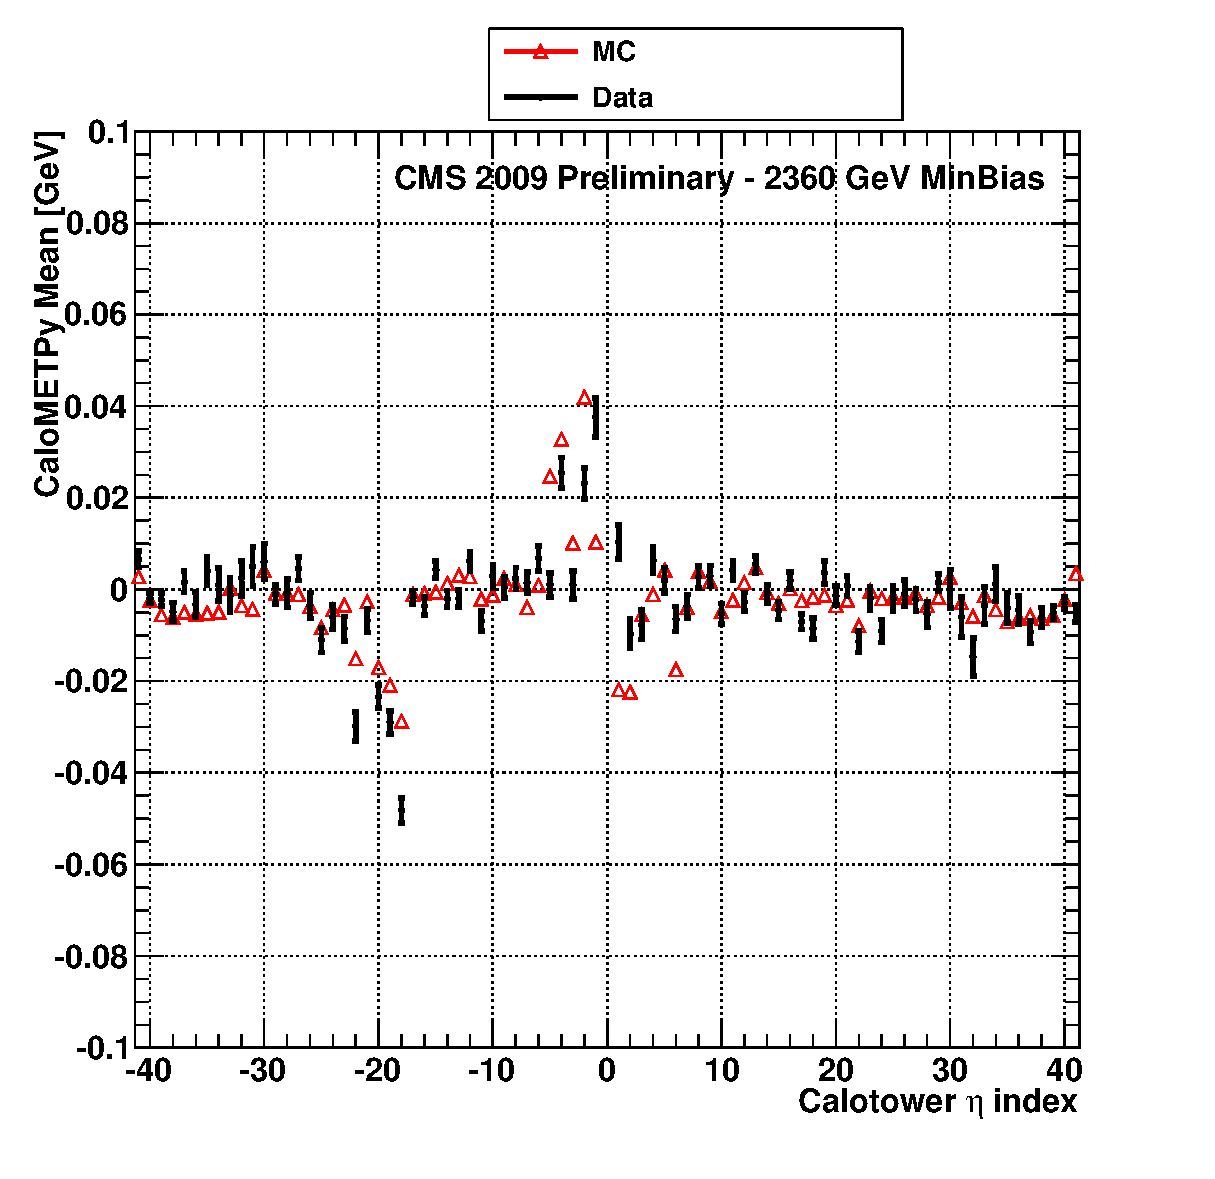
\includegraphics[width=0.5\textwidth]{plots_DataVsMC_MB_2360GeV/g_calometPyMean_vs_ieta_2360.eps} &
  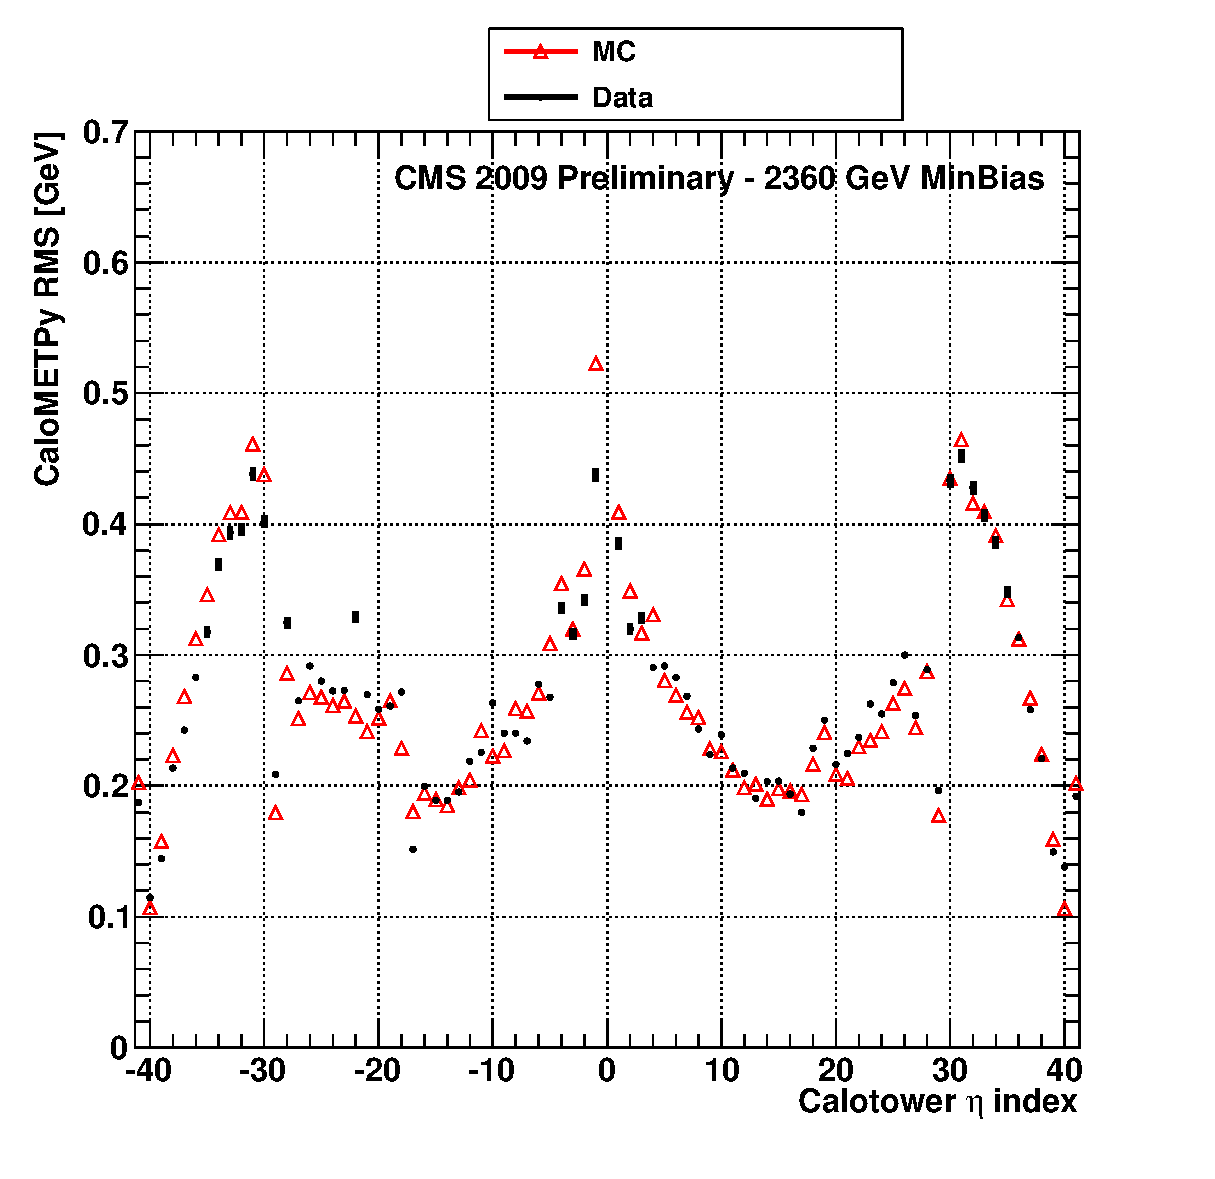
\includegraphics[width=0.5\textwidth]{plots_DataVsMC_MB_2360GeV/g_calometPyRMS_vs_ieta_2360.eps} \\
 \end{tabular}
 \caption{\small Comparison of the $\eymiss$ Mean vs. $i\eta$ of calotowers and $\eymiss$ RMS vs. $i\eta$ of calotowers between 
          data and Monte Carlo at $2360$ GeV.\label{fig:METy_MeanRMS_vs_ieta_2360}}
\end{figure}


\clearpage
